%%% آپدیت شده در خرداد 1402
%%% برای جلوگیری از نوشته شدن کتاب نامه به جای منابع و مراجع، تکس لایو ورژن را روی 2021 بزارید
%%% مواردی که نسبت به قبل بروزرسانی شده است به شرح زیر می باشد
%%% 1- بولد شدن سر فصل ها
%%% 2- اضافه شدن قابلیت
%%%    \begin{subfigure}
%%% 3-   اصلاح ترتیب شماره گذاری مراجع به ترتیب اولویت ارجاع در متن 
%%% 4- مرتب شدن فایل‌ها (قرار گرفتن عکس ها و فونت ها در پوشه ای جداگانه)
%%% 5- اضافه شدن پکیج فرض
%%% 6- اضافه شدن فونت یاس برای فارسی شدن اعداد
%%% 7- اضافه شدن پکیج تنظیم سایز جدول



%%%  کلاس AUTthesis، نسخه آبان 1397
%%%   دانشگاه صنعتی امیرکبیر                 http://www.aut.ac.ir
%%%  تالار گفتگوی پارسی‌لاتک،       http://forum.parsilatex.com
%%%   آپدیت شده در آبان 95
%%%   پشتیبانی و راهنمایی          badali_farhad@yahoo.com
%%%
%%%   بازبینی و اصلاح شده در آبان ماه 1397
%%%  Tested via TeXstudio in TeXlive 2014-2018.
%%%

%-----------------------------------------------------------------------------------------------------
%        روش اجرا.: 2 بار F1 ، 2 بار  F11(به منظور تولید مراجع) ، دوبار Ctrl+Alt+I (به منظور تولید نمایه) و دو بار F1 -------> مشاهده Pdf
%%%%%%%%%%%%%%%%%%%%%%%%%%%%%%%%%%%%%%%%%%%%%%%%%%%%%%
%   TeXstudio as your IDE
%%  برای compile در TeXstudio تنها کافی است منوی Options->Configure TeXstudio را زده و در پنجره Configure TeXstudio در بخش Build گزینه Default Compiler را به XeLaTeX تغییر دهید. سند شما به راحتی compile خواهد شد.
%   F1 & F5 : Build & view
%   F6      : Compile
%   F7      : View
%   --------------
%%%%%%%%%%%%%%%%%%%%%%%%%%%%%%%%%%%%%%%%%%%%%%%%%%%%%%
%        اگر قصد نوشتن رساله دکتری را دارید، در خط زیر به جای msc،
%      کلمه phd را قرار دهید. کلیه تنظیمات لازم، به طور خودکار، اعمال می‌شود.
%%% !TEX TS-program = XeLaTeX
\documentclass[oneside,bsc,12pt]{AUTthesis}
%       فایل commands.tex را حتماً به دقت مطالعه کنید؛ چون دستورات مربوط به فراخوانی بسته زی‌پرشین 
%       و دیگر بسته‌ها و ... در این فایل قرار دارد و بهتر است که با نحوه استفاده از آنها آشنا شوید. توجه شود برای نسخه نهایی پایان‌نامه حتماً hyperref را 
%        غیرفعال کنید.


% در این فایل، دستورها و تنظیمات مورد نیاز، آورده شده است.
%-------------------------------------------------------------------------------------------------------------------
% در ورژن جدید زی‌پرشین برای تایپ متن‌های ریاضی، این سه بسته، حتماً باید فراخوانی شود.
\usepackage{float} % Required for the [H] option
\usepackage{amsthm,amssymb,amsmath,amsfonts}
% بسته‌ای برای تنطیم حاشیه‌های بالا، پایین، چپ و راست صفحه
\usepackage[top=30mm, bottom=30mm, left=25mm, right=30mm]{geometry}
% بسته‌‌ای برای ظاهر شدن شکل‌ها و تصاویر متن
\usepackage{graphicx}
\usepackage{color}
%بسته‌ای برای تنظیم فاصله عمودی خط‌های متن
\usepackage{setspace}
\usepackage{titletoc}
\usepackage{tocloft}
%با فعال کردن بسته زیر فوت‌نوت‌ها در هر صفحه ریست می‌شوند. حالت پیش‌فرض آن ریست شدن در هر فصل می‌باشد.
%\usepackage[perpage]{footmisc}
\usepackage{enumitem}
\usepackage{multirow,adjustbox}
%\usepackage{titlesec}
% بسته‌ و دستوراتی برای ایجاد لینک‌های رنگی با امکان جهش
\usepackage[pagebackref=false,colorlinks,linkcolor=blue,citecolor=red]{hyperref}
\usepackage[nameinlink]{cleveref}%capitalize,,noabbrev
 \AtBeginDocument{%
    \crefname{equation}{برابری}{equations}%
    \crefname{chapter}{فصل}{chapters}%
    \crefname{section}{بخش}{sections}%
    \crefname{appendix}{پیوست}{appendices}%
    \crefname{enumi}{مورد}{items}%
    \crefname{footnote}{زیرنویس}{footnotes}%
    \crefname{figure}{شکل}{figures}%
    \crefname{table}{جدول}{tables}%
    \crefname{theorem}{قضیه}{theorems}%
    \crefname{lemma}{لم}{lemmas}%
    \crefname{corollary}{نتیجه}{corollaries}%
    \crefname{proposition}{گزاره}{propositions}%
    \crefname{definition}{تعریف}{definitions}%
    \crefname{result}{نتیجه}{results}%
    \crefname{example}{مثال}{examples}%
    \crefname{remark}{نکته}{remarks}%
    \crefname{note}{یادداشت}{notes}%
    \crefname{asum}{فرض}{Assumption}
}
\usepackage{subcaption}
% چنانچه قصد پرینت گرفتن نوشته خود را دارید، خط بالا را غیرفعال و  از دستور زیر استفاده کنید چون در صورت استفاده از دستور زیر‌‌، 
% لینک‌ها به رنگ سیاه ظاهر خواهند شد که برای پرینت گرفتن، مناسب‌تر است
%\usepackage[pagebackref=false]{hyperref}
% بسته‌ لازم برای تنظیم سربرگ‌ها
\usepackage{fancyhdr}
% بسته‌ای برای ظاهر شدن «مراجع»  در فهرست مطالب
\usepackage[nottoc]{tocbibind}
% دستورات مربوط به ایجاد نمایه
\usepackage{makeidx,multicol}
\setlength{\columnsep}{1.5cm}

%%%%%%%%%%%%%%%%%%%%%%%%%%
\usepackage{verbatim}
\makeindex
\usepackage{sectsty}
% فراخوانی بسته زی‌پرشین و تعریف قلم فارسی و انگلیسی
\usepackage{xepersian}%[extrafootnotefeatures]
\SepMark{-}
%حتماً از تک لایو 2014 استفاده کنید.
\settextfont[Scale=1.2,Path=Fonts/,BoldFont=B Nazanin Bold.ttf]{B Nazanin.ttf}
\setlatintextfont[Path=Fonts/]{Times New Roman.ttf}
\renewcommand{\labelitemi}{$\bullet$}
%%%%%%%%%%%%%%%%%%%%%%%%%%
% چنانچه می‌خواهید اعداد در فرمول‌ها، انگلیسی باشد، خط زیر را غیرفعال کنید.
%
\setdigitfont[Scale=1.1,Path=Fonts/,BoldFont=Yas Bd.ttf]{Yas.ttf}%%Yas
%%%%%%%%%%%%%%%%%%%%%%%%%%
% تعریف قلم‌های فارسی اضافی برای استفاده در بعضی از قسمت‌های متن
\defpersianfont\nastaliq[Scale=2,Path=Fonts/]{IranNastaliq.ttf}
\defpersianfont\chapternumber[Scale=3,Path=Fonts/,BoldFont=B Nazanin Bold.ttf]{B Nazanin.ttf}
%\chapterfont{\centering}%
%%%%%%%%%%%%%%%%%%%%%%%%%%
% دستوری برای تغییر نام کلمه «اثبات» به «برهان»
\renewcommand\proofname{\textbf{برهان}}

% دستوری برای تغییر نام کلمه «کتاب‌نامه» به «منابع و مراجع«
\renewcommand{\bibname}{منابع و مراجع}


% Headings for every page of ToC, LoF and Lot
\setlength{\cftbeforetoctitleskip}{-1.2em}
\setlength{\cftbeforelottitleskip}{-1.2em}
\setlength{\cftbeforeloftitleskip}{-1.2em}
\setlength{\cftaftertoctitleskip}{-1em}
\setlength{\cftafterlottitleskip}{-1em}
\setlength{\cftafterloftitleskip}{-1em}
%%\makeatletter
%%%%\renewcommand{\l@chapter}{\@dottedtocline{1}{1em\bfseries}{1em}}
%%%%\renewcommand{\l@section}{\@dottedtocline{2}{2em}{2em}}
%%%%\renewcommand{\l@subsection}{\@dottedtocline{3}{3em}{3em}}
%%%%\renewcommand{\l@subsubsection}{\@dottedtocline{4}{4em}{4em}}
%%%%\makeatother


\newcommand\tocheading{\par عنوان\hfill صفحه \par}
\newcommand\lofheading{\hspace*{.5cm}\figurename\hfill صفحه \par}
\newcommand\lotheading{\hspace*{.5cm}\tablename\hfill صفحه \par}

\renewcommand{\cftchapleader}{\cftdotfill{\cftdotsep}}
\renewcommand{\cfttoctitlefont}{\hspace*{\fill}\LARGE\bfseries}%\Large
\renewcommand{\cftaftertoctitle}{\hspace*{\fill}}
\renewcommand{\cftlottitlefont}{\hspace*{\fill}\LARGE\bfseries}%\Large
\renewcommand{\cftafterlottitle}{\hspace*{\fill}}
\renewcommand{\cftloftitlefont}{\hspace*{\fill}\LARGE\bfseries}
\renewcommand{\cftafterloftitle}{\hspace*{\fill}}

%%%%%%%%%%%%%%%%%%%%%%%%%%
% تعریف و نحوه ظاهر شدن عنوان قضیه‌ها، تعریف‌ها، مثال‌ها و ...
%برای شماره گذاری سه تایی قضیه ها
\theoremstyle{definition}
\newtheorem{definition}{تعریف}[section]
\newtheorem{remark}[definition]{نکته}
\newtheorem{note}[definition]{یادداشت}
\newtheorem{example}[definition]{نمونه}
\newtheorem{question}[definition]{سوال}
\newtheorem{remember}[definition]{یاداوری}
\theoremstyle{theorem}
\newtheorem{theorem}[definition]{قضیه}
\newtheorem{lemma}[definition]{لم}
\newtheorem{proposition}[definition]{گزاره}
\newtheorem{corollary}[definition]{نتیجه}
\newtheorem{asum}[definition]{فرض}
%%%%%%%%%%%%%%%%%%%%%%%%
%%%%%%%%%%%%%%%%%%%
%%% برای شماره گذاری چهارتایی قضیه ها و ...
%%\newtheorem{definition1}[subsubsection]{تعریف}
%%\newtheorem{theorem1}[subsubsection]{قضیه}
%%\newtheorem{lemma1}[subsubsection]{لم}
%%\newtheorem{proposition1}[subsubsection]{گزاره}
%%\newtheorem{corollary1}[subsubsection]{نتیجه}
%%\newtheorem{remark1}[subsubsection]{نکته}
%%\newtheorem{example1}[subsubsection]{مثال}
%%\newtheorem{question1}[subsubsection]{سوال}

%%%%%%%%%%%%%%%%%%%%%%%%%%%%

% دستورهایی برای سفارشی کردن صفحات اول فصل‌ها
\makeatletter
\newcommand\mycustomraggedright{%
 \if@RTL\raggedleft%
 \else\raggedright%
 \fi}
\def\@makechapterhead#1{%
\thispagestyle{style1}
\vspace*{20\p@}%
{\parindent \z@ \mycustomraggedright
\ifnum \c@secnumdepth >\m@ne
\if@mainmatter

\bfseries{\Huge \@chapapp}\small\space {\chapternumber\thechapter}
\par\nobreak
\vskip 0\p@
\fi
\fi
\interlinepenalty\@M 
\Huge \bfseries #1\par\nobreak
\vskip 120\p@

}

%\thispagestyle{empty}
\newpage}
\bidi@patchcmd{\@makechapterhead}{\thechapter}{\tartibi{chapter}}{}{}
\bidi@patchcmd{\chaptermark}{\thechapter}{\tartibi{chapter}}{}{}
\makeatother

\pagestyle{fancy}
\renewcommand{\chaptermark}[1]{\markboth{\chaptername~\tartibi{chapter}: #1}{}}

\fancypagestyle{style1}{
\fancyhf{} 
\fancyfoot[c]{\thepage}
\fancyhead[R]{\leftmark}%
\renewcommand{\headrulewidth}{1.2pt}
}


\fancypagestyle{style2}{
\fancyhf{}
\fancyhead[R]{چکیده}
\fancyfoot[C]{\thepage{}}
\renewcommand{\headrulewidth}{1.2pt}
}

\fancypagestyle{style3}{%
  \fancyhf{}%
  \fancyhead[R]{فهرست نمادها}
  \fancyfoot[C]{\thepage}%
  \renewcommand{\headrulewidth}{1.2pt}%
}

\fancypagestyle{style4}{%
  \fancyhf{}%
  \fancyhead[R]{فهرست جداول}
  \fancyfoot[C]{\thepage}%
  \renewcommand{\headrulewidth}{1.2pt}%
}

\fancypagestyle{style5}{%
  \fancyhf{}%
  \fancyhead[R]{فهرست اشکال}
  \fancyfoot[C]{\thepage}%
  \renewcommand{\headrulewidth}{1.2pt}%
}

\fancypagestyle{style6}{%
  \fancyhf{}%
  \fancyhead[R]{فهرست مطالب}
  \fancyfoot[C]{\thepage}%
  \renewcommand{\headrulewidth}{1.2pt}%
}

\fancypagestyle{style7}{%
  \fancyhf{}%
  \fancyhead[R]{نمایه}
  \fancyfoot[C]{\thepage}%
  \renewcommand{\headrulewidth}{1.2pt}%
}

\fancypagestyle{style8}{%
  \fancyhf{}%
  \fancyhead[R]{منابع و مراجع}
  \fancyfoot[C]{\thepage}%
  \renewcommand{\headrulewidth}{1.2pt}%
}
\fancypagestyle{style9}{%
  \fancyhf{}%
  \fancyhead[R]{واژه‌نامه‌ی فارسی به انگلیسی}
  \fancyfoot[C]{\thepage}%
  \renewcommand{\headrulewidth}{1.2pt}%
}
%


%دستور حذف نام لیست تصاویر و لیست جداول از فهرست مطالب
\newcommand*{\BeginNoToc}{%
  \addtocontents{toc}{%
    \edef\protect\SavedTocDepth{\protect\the\protect\value{tocdepth}}%
  }%
  \addtocontents{toc}{%
    \protect\setcounter{tocdepth}{-10}%
  }%
}
\newcommand*{\EndNoToc}{%
  \addtocontents{toc}{%
    \protect\setcounter{tocdepth}{\protect\SavedTocDepth}%
  }%
}
\newcounter{savepage}
\renewcommand{\listfigurename}{فهرست اشکال}
\renewcommand{\listtablename}{فهرست جداول}
%\renewcommand\cftsecleader{\cftdotfill{\cftdotsep}}
%%%%%%%%%%%%%%%%%%%%%%%%%%%%%
%%%%%%%%%%%%%%%%%%%%%%%%%%%%

\begin{document}
\baselineskip=.75cm
\linespread{1.75}
%% -!TEX root = AUTthesis.tex
% در این فایل، عنوان پایان‌نامه، مشخصات خود، متن تقدیمی‌، ستایش، سپاس‌گزاری و چکیده پایان‌نامه را به فارسی، وارد کنید.
% توجه داشته باشید که جدول حاوی مشخصات پروژه/پایان‌نامه/رساله و همچنین، مشخصات داخل آن، به طور خودکار، درج می‌شود.
%%%%%%%%%%%%%%%%%%%%%%%%%%%%%%%%%%%%
% دانشکده، آموزشکده و یا پژوهشکده  خود را وارد کنید
\faculty{دانشکده مهندسی برق}
% گرایش و گروه آموزشی خود را وارد کنید
\department{گرایش الکترونیک}
% عنوان پایان‌نامه را وارد کنید
\fatitle{محل کارآموزی
\\[.75 cm]
شرکت عصر گویش پرداز}

% نام استاد(ان) راهنما را وارد کنید
\firstsupervisor{دکتر ساناز سیدین}
% \secondsupervisor{استاد راهنمای دوم}
% نام استاد(دان) مشاور را وارد کنید. چنانچه استاد مشاور ندارید، دستور پایین را غیرفعال کنید.
\firstadvisor{دکتر حمزه بیراوند}
\name{پارسا }
% نام خانوادگی نویسنده را وارد کنید
\surname{محمدی}
%%%%%%%%%%%%%%%%%%%%%%%%%%%%%%%%%%
\thesisdate{شهریور 1402}

% چکیده پایان‌نامه را وارد کنید
\fa-abstract
{
مدل‌های بازشناسی خودکار گفتار دسته‌ای از سیستم‌های هوش مصنوعی هستند\LTRfootnote{Automatic Speech Recognition} که برای تبدیل زبان گفتاری به متن نوشتاری طراحی شده‌اند. این مدل‌ها در طیف گسترده‌ای از کاربردها، از جمله خدمات رونویسی، دستیارهای صوتی و دستگاه‌های کنترل‌شده با صدا، نقش مهمی دارند.
\newline
در این پروژه مقاله یکی از جدیدترین و بهترین مدل های بازشناسی گفتار خوانده شده و مدل آن پیاده سازی شده است. این معماری جدید \texttt{E-Branchformer} نام دارد که توانسته است به نتایج بهتری در مقایسه با مدل های \texttt{Conformer} بدست بیاورد. در این پروژه کارآموزی به منظور ایجاد یک مدل بازشناسی گفتار برای زبان فارسی، مدل  \texttt{E-Branchformer} بر روی داده های فارسی مجموعه دادگان کامن ویس\LTRfootnote{Common Voice} به عنوان مدل صوت شناسی\LTRfootnote{Acoustics} آموزش داده شده است و همچنین یک مدل زبانی ترانسفرمری نیز بر روی داده های متنی این پایگاه داده آموزش داده شده است. این مدل نهایی که ترکیب مدل صورت شانسی و زبانی می‌باشد موفق به کسب نرخ خطای کلمات \LTRfootnote{WER: Word Error Rate} 3 درصد بر روی داده های تست کامن ویس شده است که با توجه به حجم کم دادگان نتیجه بسیار خوبی می‌باشد. در مرحله بعد این مدل بر روی سرور های هاگینیگ فیس\LTRfootnote{Huggingface} پیاده سازی شده است و مدل به صورت برخط \LTRfootnote{Online} برای عموم قابل دسترس می‌باشد.}


% کلمات کلیدی پایان‌نامه را وارد کنید
\keywords{پردازش گفتار , بازشناسی گفتار فارسی, پردازش زبان طبیعی}



\AUTtitle
%%%%%%%%%%%%%%%%%%%%%%%%%%%%%%%%%%
\vspace*{7cm}
\thispagestyle{empty}
\begin{center}

\includegraphics[height=5cm,width=12cm]{Images/besm.jpg}
\end{center}
% تاییدیه دفاع
% \newpage
\thispagestyle{empty}
%\fontsize{18pt}{19pt}\selectfont

\section*{صفحه فرم ارزیابی و تصویب پایان نامه- فرم تأیید اعضاء كميته دفاع}

\fontsize{12pt}{14pt}\selectfont
%\renewcommand{\baselinestretch}{1.5}
\vspace*{1cm}
   در این صفحه فرم دفاع یا تایید و تصویب پایان نامه موسوم به فرم کمیته دفاع- موجود در پرونده آموزشی- را قرار دهید.
\vspace*{1cm}


\subsection*{نکات مهم:}
 
\begin{itemize}
\item
	نگارش پایان نامه/رساله باید به
	{\color{red}
		زبان فارسی
	}
	و بر اساس آخرین نسخه دستورالعمل و راهنمای تدوین پایان نامه های دانشگاه صنعتی امیرکبیر باشد.(دستورالعمل و راهنمای حاضر)
\item رنگ جلد پایان نامه/رساله چاپي كارشناسي، كارشناسي ارشد و دكترا  بايد به ترتيب مشكي، طوسي و سفيد رنگ باشد.  
\item چاپ و صحافی پایان نامه/رساله بصورت
{\color{red}
	پشت و رو(دورو)
}
بلامانع است و انجام آن توصيه مي شود. 
\end{itemize}
%%%%%%%%%%%%%%%%%%%%%%%%%%%%%%%%%%%%%%%%%%%%%%%%%%%%%%%%%%%%%%%%%%%%%%%%%%%%%%%%%%%%%%%%%%%%%%%%%%
%%%%%%%%%%%%%%%%%%%%%%%%%%%%%%%%%%%%%%%%%%%%%%%%%%%%%%%%%%%%%%%%%%%%%%%%%%%%%%%%%%%%%%%%%%%%%%%%%%
\newpage
\thispagestyle{empty}
\begin{picture}(50,50)
  \put(17,0){
\includegraphics[scale=1.1]{fa-logo.png}}
  \put(4.5,-13){\footnotesize{دانشگاه صنعتی امیرکبیر}}
  \put(10.5,-27){\footnotesize{(پلی‌تکنیک تهران)}}
  \put(170,30){\bf{به نام خدا}}
  \put(140,-5){\Large\bf{تعهدنامه اصالت اثر}}
  \put(310,0){تاریخ: \datethesis}
\end{picture}

\vspace*{2.5cm}

اينجانب {\bf{\fname\lname}} متعهد می‌شوم که مطالب مندرج در این پایان‌نامه حاصل کار پژوهشی اینجانب تحت نظارت و راهنمایی اساتید دانشگاه صنعتی امیرکبیر بوده و به دستاوردهای دیگران که در این پژوهش از آنها استفاده شده است مطابق مقررات و روال متعارف ارجاع و در فهرست منابع و مآخذ ذکر گردیده است. این پایان‌نامه قبلاً برای احراز هیچ مدرک هم‌سطح یا بالاتر ارائه نگردیده است.

در صورت اثبات تخلف در هر زمان، مدرک تحصیلی صادر شده توسط دانشگاه از درجه اعتبار ساقط بوده و دانشگاه حق پیگیری قانونی خواهد داشت.


کلیه نتایج و حقوق حاصل از این پایان‌نامه متعلق به دانشگاه صنعتی امیرکبیر می‌باشد. هرگونه استفاده از نتایج علمی و عملی، واگذاری اطلاعات به دیگران یا چاپ و تکثیر، نسخه‌برداری، ترجمه و اقتباس از این پایان نامه بدون موافقت کتبی دانشگاه صنعتی امیرکبیر ممنوع است. 
نقل مطالب با ذکر مآخذ بلامانع است.\\
\vspace{2.5cm}


{\centerline {\bf{\fname\lname}}}
\vspace*{.2cm}
{\centerline{امضا}}
%%%%%%%%%%%%%%%%%%%%%%%%%%%%%%%%%
% چنانچه مایل به چاپ صفحات «تقدیم»، «نیایش» و «سپاس‌گزاری» در خروجی نیستید، خط‌های زیر را با گذاشتن ٪  در ابتدای آنها غیرفعال کنید.
% پایان‌نامه خود را تقدیم کنید
% نیایش خود را در فایل زیر بنویسید.
% \begin{acknowledgementpage}

\vspace{1.5cm}

{\nastaliq
{
اينجانب پارسا محمدی مراتب امتنان و تشكر خود را نسبت به استاد كارآموزي جناب دكتر ساناز سیدین و سرپرست محترم کارآموزی دکتر بیراوند كه در گذراندن اين دوره كارآموزي همواره مرا ياري نموده اند، ابراز مي دارم.
}}\end{acknowledgementpage}
\newpage
% سپاسگزاری را در فایل زیر بنویسید.

%%%%%%%%%%%%%%%%%%%%%%%%%%%%%%%%%%%%
\newpage\thispagestyle{empty}
% سپاس‌گزاری
{\nastaliq
سپاس‌گزاری
}
\\[2cm]

{\nastaliq
اينجانب پارسا محمدی مراتب امتنان و تشكر خود را نسبت به استاد كارآموزي 
دكتر ساناز سیدین و سرپرست محترم کارآموزی دکتر حمزه بیراوند كه در گذراندن اين دوره كارآموزي همواره مرا ياري نموده اند، ابراز مي دارم.
}








% با استفاده از دستور زیر، امضای شما، به طور خودکار، درج می‌شود.
\signature








%%%%%%%%%%%%%%%%%%%%%%%%%%%%%%%%%%%%%%%%%
%%%%%%%%%%%%%%%%%%%%%%%%%%%%%%%%%کدهای زیر را تغییر ندهید.
\newpage\clearpage

\pagestyle{style2}

\vspace*{-1cm}
\section*{\centering چکیده}
%\addcontentsline{toc}{chapter}{چکیده}
\vspace*{.5cm}
\ffa-abstract
\vspace*{2cm}


{\noindent\large\textbf{واژه‌های کلیدی:}}\par
\vspace*{.5cm}
\fkeywords
% دستور زیر برای شماره گذاری صفحات قبل از فصل اول با حروف ابجد است.
\pagenumbering{alph}
%-----------------------------------------------------------------------------
% فایل زیر دستورات مربوط به نمایش صفحات فهرست مطالب- فهرست اشکال و جداول است.
%{\pagestyle{style2}
%\tableofcontents}\newpage
%
%\listoffigures
\cleardoublepage
\pagestyle{style6}
\tableofcontents
\pagestyle{style6}
\cleardoublepage
%اگر لیست تصاویر و لیست جداول ندارید ، کدهای زیر را با گذاشتن % در ابتدای آنها، غیرفعال کنید.
\BeginNoToc
%============
\addtocontents{lof}{\lofheading}% add heading to the first page in LoF
\pagestyle{style5}
\listoffigures
\thispagestyle{style5}
\cleardoublepage
%============
% \addtocontents{lot}{\lotheading}% add heading to the first page in LoT
% \thispagestyle{style4}
% \listoftables
% \thispagestyle{style4}
%============
%\cleardoublepage
%
% \cleardoublepage
% \setcounter{savepage}{\arabic{page}}
% \mainmatter
% \addtocontents{toc}{\tocheading}% add heading to the first page in ToC, after frontmatter entries
\EndNoToc
% در صورت تمایل می‌توانید با فعال کردن دستور بالا، لیست تصاویر را به  پایان‌نامه خود اضافه کنید.
%-------------------------------------------------------------------------symbols(فهرست نمادها)
% وجود لیست نمادها الزامیست.(لطفاً نمادهای خود را جایگذین نمادهای پیش‌فرض کنید.)
% %%%%%%%%%%%%%

{\centering\LARGE\textbf{فهرست نمادها}\par}%

\pagenumbering{alph}
\setcounter{page}{\thesavepage}
%\setcounter{page}{6}
\vspace*{1cm}

\pagestyle{style3}
%\thispagestyle{empty}
%\addcontentsline{toc}{chapter}{فهرست نمادها}
\symb{\text{ نماد}}{مفهوم}
\\
%مقادیر بالا را تغییر ندهید
%%%%%%%%%%%%%%%%%%%%%%%%%%%%%%%%%%%%%%%%%%%%%%%%%%%%%%%%%
\symb{\mathbb{R}^n}{
فضای اقلیدسی با بعد $n$
}
\symb{\mathbb{S}^n}{
کره یکه $n$ بعدی
}
\symb{M^m}{
خمینه $m$-بعدی $M$
}
\symb{\mathfrak{X}(M)}{
جبر میدان‌های  برداری هموار روی $M$
}
\symb{\mathfrak{X}^1(M)}{
مجموعه میدان‌های برداری هموار یکه روی $(M,g)$ 
}
\symb{\Omega^p(M)}{
مجموعه $p$-فرمی‌های روی خمینه $M$
}
\symb{Q}{
اپراتور ریچی
}
\symb{\mathcal{R}}{
تانسور انحنای ریمان
}
\symb{ric}{
تانسور ریچی
}
\symb{L}{
مشتق لی
}
\symb{\Phi}{
2-فرم اساسی خمینه تماسی
}
\symb{\nabla}{
التصاق لوی-چویتای
}
\symb{\Delta}{
لاپلاسین ناهموار
}
\symb{\nabla^*}{
عملگر خودالحاق صوری القا شده از التصاق لوی-چویتای
}
\symb{g_s}{
متر ساساکی
}
\symb{\nabla}{
التصاق لوی-چویتای وابسته به متر ساساکی
}
\symb{\Delta}{
عملگر لاپلاس-بلترامی روی $p$-فرم‌ها
}

%%%%%%%%%%%%%%%%%%%%%%%%%%%%%%%%%%%%%%%

\thispagestyle{style3}
\newpage
%\pagestyle{style1}
%%%%%%%%%%%%%%%%%%%%%%%%%%%%%%%%%%%%


\pagenumbering{arabic}
\pagestyle{style1}
%--------------------------------------------------------------------------chapters(فصل ها)
\chapter{مقدمه}
{
صوت یکی از مهم‌ترین حالات انرژی در جهان ما می‌باشد و راه ارتباطی اصلی بسیاری از انسان‌ها و دیگر موجودات،‌ از طریق سیگنال های صوتی می‌باشد. به همین دلیل، درک و پردازش این نوع از داده‌ها، اهمیت بسیاری در عصر حاضر برای ما دارا می‌باشد. 

مدل‌های تشخیص خودکار گفتار  دسته‌ای از سیستم‌های هوش مصنوعی هستند که برای تبدیل زبان گفتاری به متن نوشتاری طراحی شده‌اند. این مدل‌ها در طیف گسترده‌ای از کاربردها، از جمله خدمات رونویسی، دستیارهای صوتی و دستگاه‌های کنترل‌شده با صدا، نقش مهمی دارند. مدل‌های  از تکنیک‌های یادگیری عمیق، مانند شبکه‌های عصبی ترانسفورمر برای پردازش داده‌های صوتی و تولید رونویسی دقیق از کلمات و عبارات گفتاری استفاده می‌کنند.

تشخیص خودکار گفتار سر به سر \LTRfootnote{End to End ASR}
یک روش در تشخیص خودکار گفتار است که در آن از یک مدل شبکه عصبی واحد برای تبدیل مستقیم زبان گفتاری به متن نوشتاری بدون نیاز به اجزای میانی مانند واج یا واحدهای زبانی استفاده می‌شود. هدف مدل‌های بازشناسی گفتار سر به سر ساده‌سازی مسیر\LTRfootnote{Pipeline} بازشناسی گفتار است و به دلیل توانایی‌شان در یادگیری نگاشت‌های پیچیده گفتار به متن محبوبیت پیدا کرده‌اند. آنها اغلب مبتنی بر معماری‌های یادگیری عمیق، مانند شبکه‌های عصبی مکرر \LTRfootnote{RNN: Recurrent Neural Network} یا ترانسفورماتورها هستند، و در دستیابی به نتایج رقابتی در تسک های تشخیص گفتار، نویدبخش نشان داده‌اند، و آنها را برای برنامه‌هایی مانند خدمات رونویسی، دستیارهای صوتی و غیره ارزشمند می‌سازند.

در شرکت عصر گویش پرداز کار مشابه‌ای در زمینه بازشناسی گفتار قبلا انجام شده است. در حال حاظر نرم افزار نویسا شرکت عصر گویش پرداز برای کاربرد های تجاری بازشناسی گفتار استفاده می‌شود. اما محدودیت نرم افزار فعلی نویسا این است که این نرم افزار با مدل های ان گرام\LTRfootnote{Ngram} آموزش داده شده است و روش های
تعبیه‌سازی کلمات\LTRfootnote{Word Embedding}
برای آموش این مدل استفاده شده است؛ مدل فعلی در درک اسامی خاص و کلمات پیچیده ضعیف عمل می‌کند زیرا در دیکشینری آن کلمه خاص ممکن است موجود نباشد. اما مدل های 
خودنگرش\LTRfootnote{Self Attention}
به روش های تعبیه سازی نیاز ندارند و خودشان می‌توانند ارزش کلمات را در جملات درک کنند. پروژه من آموزش یک مدل 
سر به سر بازشناسی گفتار فارسی
می‌باشد که دارای معماری 
خودنگرش
‌باشد.

در مطالعاتی که در این دوره کارآموزی انجام گرفت چند مقاله به منظور یافتن بهترین معماری برای تشخیص گفتار فارسی بررسی شد؛ یکی از بهترین کاندیدا ها مدل \texttt{Whisper} شرکت \texttt{AI Open} می‌باشد. این مدل توانایی بازشناسی گفتار به زبان های مختلف دارد، اما دقت خروجی آن برای زبان فارسی کم است. شرکت عصرگویش پرداز قبلا برای فاین تیون\LTRfootnote{Fine Tune} کردن این مدل اقدام کرده است اما با توجه به ماهیت 
نیمه نظارتی \LTRfootnote{Semi-Supervised}
این مدل خروجی مدل فاین توین شده مناسب نبود. با همفکری که در شرکت صورت گرفت تصمیم بر این شد که از مدل های \texttt{Conformer} یا \texttt{Branchformer} برای آموزش مدل بازشناسی گفتار فارسی استفاده شود.

در ادامه، در فصل دوم به معرفي شركت عصرگويش پرداز پرداخته و بخشي از مهم ترين محصولات و زمينه هاي فعاليت اين شركت بررسي خواهند شد همچنین به معرفی این پروژه کارآموزی خواهیم پرداخت. در فصل سوم و چهارم، تجربيات كسب شده در اين دوره كارآموزي سه ماهه، بيان خواهد شد و برخي از چالش ها و راه حل هايي كه در اين دوره ارائه شدند، بررسي خواهند شد. در فصل سوم به مباحث تئوری پروژه از جمله مدل انتخابی و دادگان اشاره خواهد شد و در فصل چهارم به تجربیات عملی و چالش های آموزش و پیاده سازی اشاره مدل اشاره خواهد شد. در نهايت در فصل پنجم، نتيجه گيري مربوط به اين دوره كارآموزي بيان خواهد شد و پيشنهاد هايي در جهت بهبود خروجی مدل ارائه شده، ذكر خواهد شد.
}
\chapter{معرفی محل کارآموزی و پروژه کارآموزی}

در این قسمت، به طور مختصر، شرکت عصرگویش‌پرداز معرفی شده و در ادامه محصولات اصلی شرکت و همچنین زمینه‌های فعالیت این شرکت ذکر خواهند شد.

\section{معرفی شرکت}

عصر گویش پرداز (سهامی خاص) فعال‌ترین شرکت در زمینه هوش مصنوعی و پردازش سیگنال گفتار بوده كه فعالیت خود را از ابتدای سال ۱۳۸۲ شروع كرده است. عمده محصولات و خدمات ارائه شده توسط این شرکت برای نخستین بار در کشور و به صورت حرفه‌ای در زمینه‌های پردازش و تشخیص گفتار بوده است. این شرکت با پشتوانه فنی گروهی از متخصصان کشور از دانشگاه صنعتی شریف تأسیس شد که سابقه و تجربه پژوهشی آنها در زمینه‌های مرتبط با پردازش سیگنال به چندین سال قبل از شروع رسمی فعالیت شرکت برمی‌گردد.

\subsection{محصولات شرکت}

عصرگویش پرداز پیشرو در ارائه سیستم های مبتنی بر گفتار برای زبان فارسی، محصولات مختلفی را توسعه داده است که بیشتر آنها برای نخستین بار برای زبان فارسی انجام شده و منحصراً توسط این شرکت تولید می‌شوند. برخی از محصولات این شرکت عبارتند از:
\begin{itemize}
	\item نویسا: نخستین سامانه تایپ گفتاری فارسی
	\item نیوشا: نخستین سامانه تلفن گویای هوشمند مبتنی بر گفتار
	\item آریانا: سامانه متن به گفتار فارسی با صدای طبیعی
	\item شناسا: تعیین هویت گوینده
	\item رمزآوا: احراز هویت گوینده
	\item بینا: تصویر خوان هوشمند
	\item رومند: چت بات هوشمند
	\item جویا: سامانه جستجوی عبارات و کلمات در گفتار
	\item پوشا: سامانه پنهان سازی اطلاعات در تصویر (استگانوگرافی)
	\item پدیدا: سامانه کشف تصاویر نهان نگاری شده
	\item پارسیا: اولین نرم‌افزار متـرجم گفتار به گفتار فارسی به انگلیسی/ عربی
	\item نویسیار: اولین نرم‌افزار تایپ هوشمند فارسی
	\item کارا: نخستین سامانه تشخیص فرمان صوتی برای ویندوز
\end{itemize}

\subsection{زمینه‌های فعالیت}

این شرکت امروزه دارای گروهی متخصص و منسجم از افرادی با تخصص و تجربه بالا بوده و سابقه طولانی و موفق در زمینه تحقیق و توسعه و کاربردی کردن توانمندی های پژوهشی دارد و علاوه بر ارائه محصولات مختلف در زمینه‌های هوش مصنوعی، پردازش گفتار فارسی و انگلیسی و پردازش تصویر، قادر به انجام پروژه های مختلف و ارائه خدمات در زمینه‌های مختلف نرم‌افزاری می‌باشد. از جمله زمینه‌های فعالیت این شرکت:
\begin{itemize}
	\item تولید نرم افزارها و سخت افزارهای هوشمند
	\item هوش مصنوعی و شناسایی الگو
	\item پردازش سیگنال (گفتار و تصویر)
	\item تشخیص گفتار و تایپ گفتاری (تبدیل گفتار به متن)
	\item سنتز گفتار و متن خوان (تبدیل متن به گفتار)
	\item شناسایی افراد از روی صدا
	\item پردازش زبان طبیعی
	\item بهبود كیفیت گفتار
	\item طراحی دادگان‌های گفتاری و متنی
	\item طراحی، توسعه و پشتیبانی نرم افزارهای کاربردی مرتبط
	\item سیستم‌های تلفن گویا (با قابلیت تشخیص گفتار)
	\item سامانه‌های تلفنی مبتنی بر ویپ (استریسک، الستیکس و ...)
	\item برنامه نویسی روی ریزکامپیوترها (\lr{DSP}، تلفن همراه و ...)
\end{itemize}

با توجه به نوآوری های انجام گرفته در شركت عصرگویش پرداز، این شرکت علاوه بر انتشار مقاله‌های مختلف در نشریات و کنفرانس‌های علمی ملی و بین‌المللی، دارای افتخارات و تأییدیه‌های متعددی می‌باشد.

\section{پروژه کارآموزی}
شرکت عصر گویش پرداز هرساله در فصل تابستان تعداد محدودی کارآموز از دانشجویان بهترین دانشگاه های ایران جذب می‌کند. دانشجویانی که بعد از ارسال رزومه و قبولی در مصاحبه انتخاب می‌شوند در دوره سه ماه کارآموزی شرکت عصر گویش پرداز مشغول می‌شوند. هر کارآموز باید یک یا دو پروژه از پروژه های فعال شرکت را تکمیل کند و پس از پیاده سازی و ارائه خروجی پروژه به مسئول کارآموزی گواهی اتمام کارآموزی را دریافت می‌کند.
پروژه های کارآموزی از پروژه های فعال و حل نشده شرکت می‌باشد. دانشجویان بعد از اینکه به گروه های چند نفری تقسیم شدند بر اساس دانش و علاقه آنها یک پروژه به آنها داده می‌شود و یکی از دانشجویان ارشد هوش مصنوعی دکتر صامتی (بنیان گذار شرکت) به عنوان رییس گروه مشخص شده و مسئول هدایت دانشجویان در طول مدت کارآموزی می‌باشد.

 بعد از همفکری با استاد محترم کارآموزی دکتر سیدین و همچنین مشورت با مسئول کارآموزی شرکت پروژه بازشناسی گفتار فارسی انتخاب شد. من در طول دوره کارآموزی موظف به پیدا کردن بهترین مدل ترانسفرمری برای این امر و پیاده سازی آن بر روی سرور های شرکت بودم. مدل جدید قرار است بجای مدل قدیمی شرکت در نرم افزار نویسا قرار گیرد. در فصل بعدی به مدل انتخاب شده، معماری آن، دادگان استفاده شده و چالش های آن بیان خواهد شد. 

\chapter{مدل شبکه عصبی و دادگان}

\section{مطاله مقالات جدید}\label{sec1}

در این فصل به مباحث نظری این پروژه کارآموزی اشاره می کنیم. در این فصل بیان می شود که چرا برای این پروژه نیاز به مطاله جدید ترین مقالات حوزه 
بازشناسی گفتار
می‌باشد.
در ادامه بهترین مدل های فعلی 
بازشناسی گفتار
اشاره می شود و خلاصه ای از مقالات آنها بیان می شود ؛
و بعد از مقایسه بهترین مدل های این حوزه بیان می شود که مدل نهایی پروژه 
\texttt{\raggedright E-Branchformer}
 می‌باشد. با استفاده این مدل و دادگان
کامن ویس\LTRfootnote{Common Voice}
 مدل بازشناسی فارسی آموزش داده شده است.
در ادامه به جزئیات دادگان استفاده شده در این پروژه اشاره خواهد شد.
در فصل بعدی به جزئیات پیاده سازی و چالش های آن اشاره خواهد شد.


با توجه به اینکه هدف اصلی این پروژه کارآموزی بروزرسانی مدل فعلی استفاده شده در نرم افزار بازشناسی گفتار فارسی(نویسا) می‌باشد\LTRfootnote{\url{https://nevisalive.com/}}؛ باید جدید ترین مقالات در حوزه بازشناسی گفتار مطالعه شود تا با جدید‌ترین مدل ها و روش های باز‌شناسی گفتار آشنا شد. پس از انجام تحقیقات و مشورت با ارشد پروژه نتیجه این شد که با توجه به اینکه امروزه مدل های 
سر به سر\LTRfootnote{End to End}
بهترین نتایج را دارند از این مدل های استفاده شود. همچنین مدل های ترانسفورمری با دارای بودن خاصیت 
خودنظارتی\LTRfootnote{Self-attention}
در حجم داده های زیاد نتایج بسیار خوبی را خروجی می‌دهند. اخیرا مدل های ترانسفورمری با شبکه های کانولوشنی ترکیب شده اند این امر باعث بهبود قابل توجهی در خروجی آنها شده است.

در مطالعاتی که در این دوره کارآموزی انجام گرفت چند مقاله به منظور یافتن بهترین معماری برای تشخیص گفتار فارسی بررسی شد؛ یکی از بهترین کاندیدا ها مدل \texttt{Whisper} شرکت \texttt{AI Open} می‌باشد. این مدل توانایی بازشناسی گفتار به زبان های مختلف دارد، اما دقت خروجی آن برای زبان فارسی کم است. شرکت عصرگویش پرداز قبلا برای فاین تیون کردن این مدل اقدام کرده است اما با توجه به ماهیت 
نیمه نظارتی
این مدل خروجی مدل فاین توین شده مناسب نبود. با مطالعه و همفکری که در شرکت صورت گرفت تصمیم بر این شد که از مدل های \texttt{Conformer} یا \texttt{Branchformer} برای آموزش مدل بازشناسی گفتار فارسی استفاده شود.

\section{معماری کانفرمر}\label{sec2}
باتوجه به ویژگی های ارزشمند معماری
کانفرمر\LTRfootnote{Conformer}
در این دوره کارآموزی ابتدا مقاله این مدل خوانده شد و گزارشی از آن تهیه شد. در ادامه ویژگی های این مدل و معماری آن را مورد بررسی قرار می دهیم.

اخیراً مدل‌های مبتنی بر شبکه عصبی ترانسفورماتور و کانولوشن 
\LTRfootnote{CNN: Convolutional Neural Network}
نتایج امیدوارکننده‌ای را در تشخیص خودکار گفتار 
بازشناسی گفتار
نشان داده‌اند که عملکرد بهتری از شبکه‌های عصبی بازگشتی 
دارد. مدل‌های ترانسفورماتور در ثبت تعاملات جهانی 
\LTRfootnote{Global Optima}
مبتنی بر محتوا خوب هستند، در حالی که 
\verb;CNN;
ها از ویژگی‌های محلی به طور موثر بهره‌برداری می‌کنند. ترکیب این دو مدل باعث می‌شود که هم ویژگی های محلی و هم جهانی به خوبی استخراج شود. مدل 
کانفرمر
به واسطه معماری خاص خود توانسته است که ویژگی ترانسفورماتور ها و کانولوشن ها را با هم ترکیب کند، و هم در دنباله های کوتاه و بلند داده ها به خوبی عمل کنند. \cite{gulati2020conformer}

معماری مدل کانفورمر
مانند دیگر مدل های سر به سر ترانسفورمری
می‌باشد.
 این مدل از یک بخش
رمزگزار\LTRfootnote{Encoder}
و یک بخش
رمزگشا\LTRfootnote{Decoder}
تشکیل شده است.
این دو بخش توسط جوینت های 
\verb|CTC|
به هم متصل شده اند.
مدل ترانسفورمر در سال 2017 توسط مقاله
\texttt{\raggedright {need you all attention}}
منتشر شد. \cite{DBLP:journals/corr/VaswaniSPUJGKP17}

همین طور که در تصویر 
\ref{fig:transformer}
مشخص است معماری ترانسفورمر ها از بخش های رمزگذار و رمزگشا تشکیل شده است و
تفاوت معماری کانفرمر و ترانسفرمر عادی در ورودی مدل و بخش رمزگذار می‌باشد. در رمزگذار 
 از ترکیب شبکه های کانولوشنی و ترانسفورمری استفاده شده است که این امر این مدل را قادر می سازد درک بهتری از ویژگی های متن ورودی بدست بیاورد.
 
\begin{figure}[H]
  \centering
  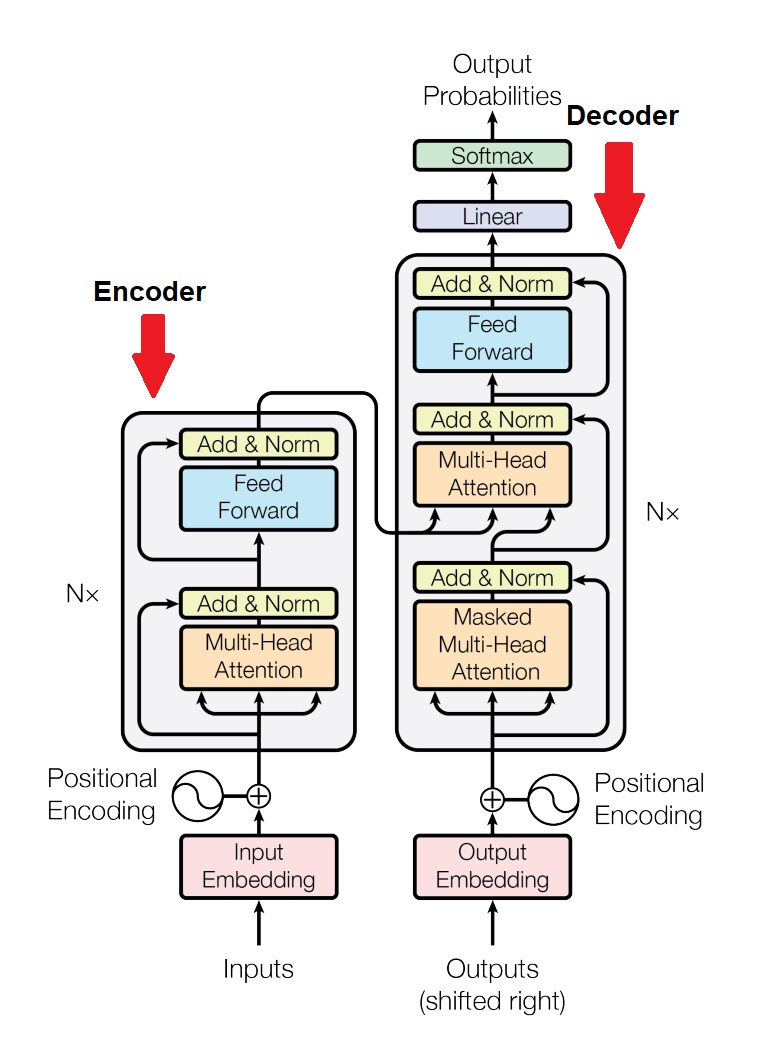
\includegraphics[width=0.6\textwidth, height=13cm]{Images/Chapter2/transformer.jpg}
  \caption{تصویر معماری مدل ترانسفورمر. این مدل از یک بخش رمزگذار و رمزگشا تشکیل شده است و بخش های آن توسط فلش در تصویر مشخص است.}
  \label{fig:transformer}
\end{figure}

 همان طور که از تصویر \ref{fig:conformer}
مشخص است.
بلاک کانقرمر یک ماژول 
  \verb|Forward Feed|
  و بعد از آن ماژول 
  خود نظارتی
  آمده است.
  سپس خروجی این ماژول وارد ماژول  کانولوشن می شوند
  در نهایت نیمی از ابعاد  وارد 
  \verb|Forward Feed|
  می شود.
  در مرحله آخر یک بلوک 
  \verb|Layernorm|
  قرار داده شده است.
  
 \begin{figure}[H]
  \centering
  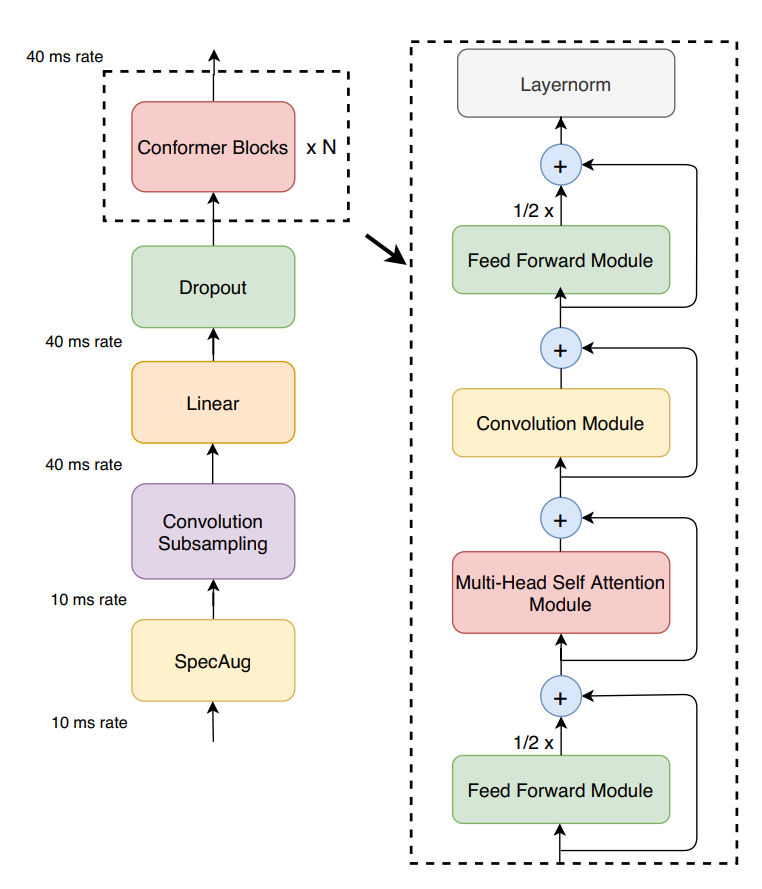
\includegraphics[width=0.5\textwidth,height=9cm]{Images/Chapter2/conformer.png}
  \caption{
  معماری رمزگذار کانفرمر. 
  }
  \label{fig:conformer}
\end{figure}



همان طور که پیش تر گفته شد این امر معماری کانفرمر را قادر می سازد که هم ویژگی های جهانی و هم ویژگی های محلی را به خوبی تشخیص بدهد. این معماری عالی معماری کانفرمر را به یکی از بهترین مدل های موجود برای کار های 
بازشناسی گفتار
تبدیل کرده است.
این مدل یکی از بهترین کاندیدا های مدل 
بازشناسی گفتار فارسی
بود. من در این دوره کارآموزی مقاله کانفرمر را مطاله کردم و چند پیاده سازی از آن را بررسی کردم. مقاله خوانده شده در یک جلسه برای اعضای بخش تحقیقات و توسعه\LTRfootnote{Research and Development} شرکت معرفی شد و نظرات آنها در مورد این مدل دریافت شد.
این مدل با تمام ویژگی های خوب آن اندکی قدیمی شده است و مدل های جدید تر وجود دارند که ادعا می کنند به نتایج بهتری دست یافته اند.
در بخش بعدی به یکی از بهترین آنها اشاره می شود.

\section{معماری ای-برانچفرمر}
یکی از جدید ترین معماری های ارائه شده در حوزه 
بازشناسی گفتار
معماری 
ای-برانچفرمر\LTRfootnote{E-Branchformer}
می‌باشد.

این مدل که در کنفراس
\verb|Interspeech|
سال 2023
معرفی شد و نتایج خوبی که بر روی دیتاست های مختلف بدست آورد توجه های زیادی را بخودش جلب کرده است.

مدل
\texttt{\raggedright E-Branchformer}
بهبود یافته مدل 
\texttt{\raggedright Branchformer}
می‌باشد.\cite{kim2022ebranchformer}
حرف 
\verb|E|
مخفف کلمه
\verb|Enhanced|
می‌باشد که به معنای تقویت شده می‌باشد و ای-برانچفرمر تقویت شده مدل برانچفرمر می‌باشد.
برانچفرمر های ساختاری بسیار مشابه به کانفرمر ها دارند. در برانچفرمر ها نیز فقط معماری بخش رمزگذار با  معماری ترانسفر ها متفاوت است، در رمزگذار آن مانند کانفرمر ترکیبی از بلوک های کانفرمری و 
خود نظارتی
استفاده می شود تا هم ویژگی های محلی و هم جهانی داده ها به خوبی توسط مدل درک شود.

تفاوت اصلی کانفرمر و برانچفرمر در نوع ترکیب بلوک های 
کانفرمری و 
خود نظارتی
می‌باشد.
در برانچفمر ها تلاش شده است که این ترکیب به صورت موازی انجام شود، در حالی که در کانفرمر این ترکیب به صورت سری انجام شده است این امر در شکل \ref{fig:conformer} مشخص است. 
موازی سازی انجام شده در برانچفرمر ها باعث می شود که عمق شبکه عصبی کمتر شود و راحت تر به نقطه بهینه همگرا شود.
همچنین تعداد پارامتر های استفاده شده در برانچفرمر در تعداد لایه های برابر کمتر از کانفرمر ها می‌باشد، که امر باعث کاهش هزنیه محاسباتی آموزش این مدل می شود.

 \begin{figure}[H]
  \centering
  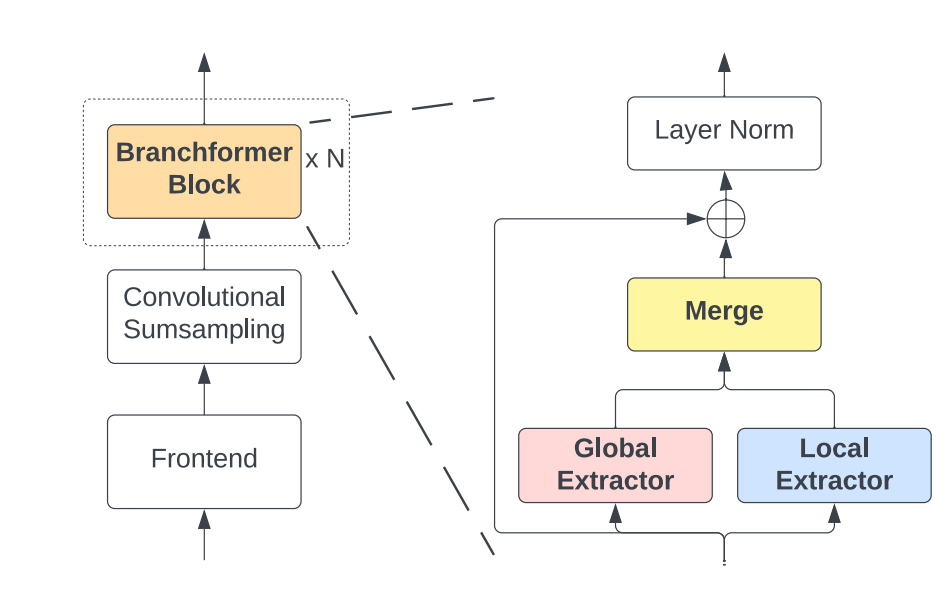
\includegraphics[height=6cm]{Images/Chapter2/EBranchformer.png}
  \caption{
  معماری رمزگذار برانچفرمر.
  }
  \label{fig:EBranchformer}
\end{figure}

شکل \ref{fig:EBranchformer}
معماری رمزگذار برانچفرمر را نمایش می دهد. همین طور که مشخص است نیمی از ابعاد داده ها به استخراج کننده محلی\LTRfootnote{Local} و نیم دیگر به استخراج کننده جهانی داده می شود. این نوع معماری خاص مدل را قادر می سازد که هم ویژگی های محلی و هم ویژگی های جهانی\LTRfootnote{Global} را به خوبی تشخیص دهد و مدل هم در دنباله\LTRfootnote{Sequence} داده های کوتاه و هم در دنباله داده های بلند خوب عمل کند.

تفاوت 
برانچفرمر
و
ای-برانچفرمر
این نوع ترکیب این دو بخش موازی می‌باشد.
ای-برانچفرمر بسیار بهینه تر با این دو بخش را باهم ترکیب می‌کند.
در ادامه برای یافتن بهترین مدل برای 
بازشناسی گفتار
باید مطالعه ای صورت بپذیرد که بهترین مدل ممکن برای آموزش استفاده شود.
در بخش بعدی به مطالعه مقاله ای پرداخته می شود که این دو مدل برتر یعنی ای-برانچفرمر و کانفرمر را با هم مقایسه کرده است و بهترین مدل را معرفی کرده است.



\section{مقایسه ای-برانچفرمر و کانفرمر}\label{sec4}

اخیرا مقاله ای چاپ در چاپ شده است که دو مدل برتر ای-برانچفرمر و کانفرمر را باهم مقایسه می‌کند.\cite{peng2023comparative}
این مقاله این دو مدل را در سه تا از تسک های گفتار بازشناسی گفتار، ترجمه گفتار و درک گفتار بررسی می‌کند. مقایسه در تعدادی از بزرگترین و معروف ترین دیتاست های منبع باز صورت گرفته است؛ و خروجی های این مدل ها بر روی این دیتاست ها با هم مقایسه شده اند.

 \begin{figure}[H]
  \centering
  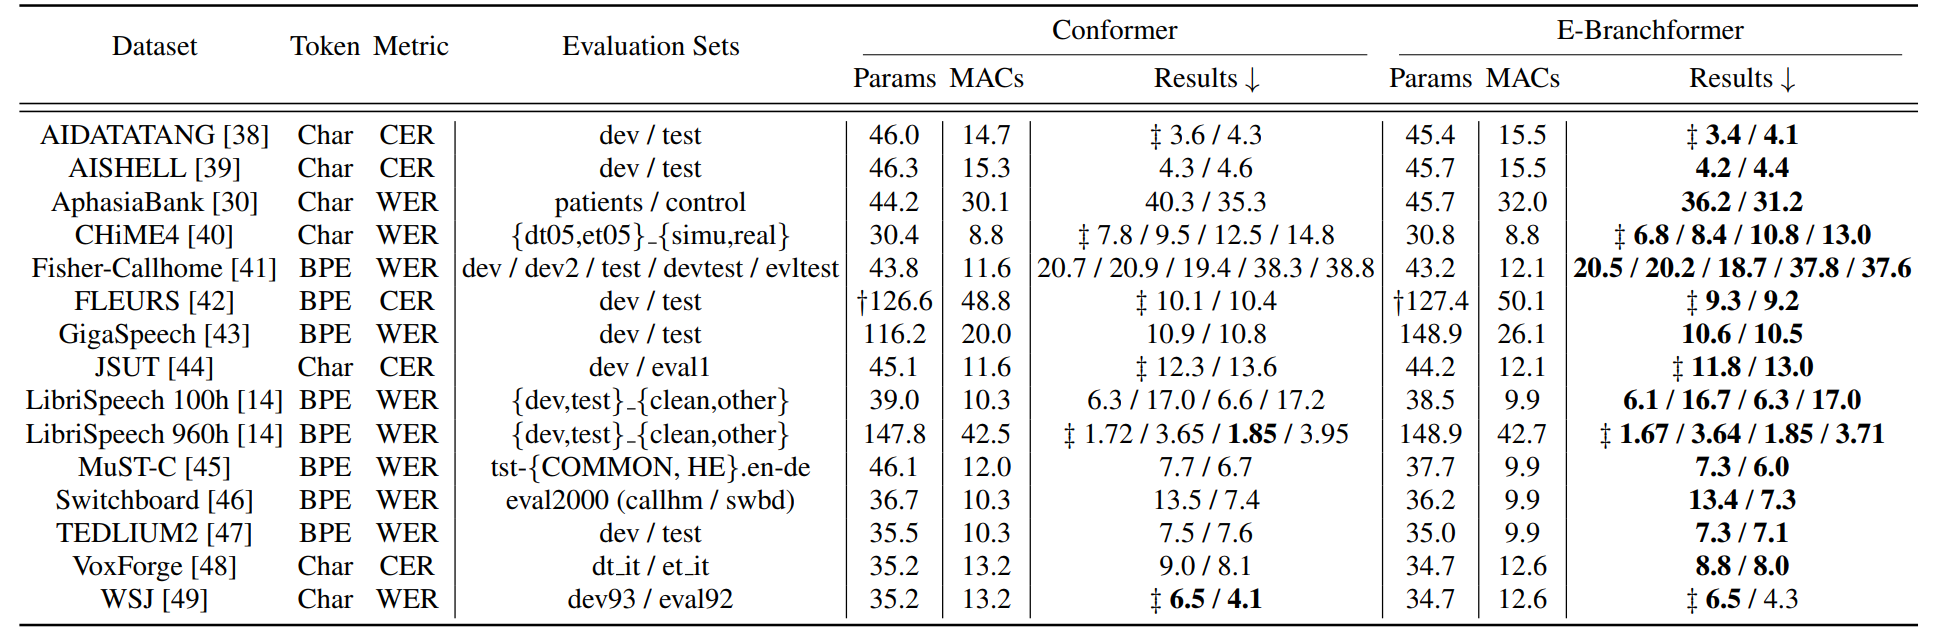
\includegraphics[width=1\textwidth,height=6cm]{Images/Chapter2/confvsbranch.png}
  \caption{
  جدول مقایسه کننده دو مدل کانفرمر و ای-برانچفرمر. این دو مدل در 12 دیتاست با هم مقایسه شده اند.
  }
  \label{fig:confvsbranch}
\end{figure}

همین طور که در تصویر \ref{fig:confvsbranch}
مشخص است مدل ای-برانچفرمر نتایج بسیار بهتری نسبت به کانفرمر در اکثر دادگان بدست آورده است.
این جدول و جداول دیگری که در این دو مدل را در تسک های مختلف مقایسه می کنند نشان می‌دهند که مدل ای-برانچفرمر نتایج بسیار بهتری نسبت به کانفرمر در هر سه تسک گفتار بدست آورده است. این مقاله بر برتری ای-برانچفرمر تأکید می‌کند زیرا معماری موازی شده رمزگذار آن باعث بهبود نتایج و کاهش هزینه محاسباتی شده است.

با توجه به نتایج بهتر مدل ای-برانچفرمر بعد از مشورت هایی که در گروه انجام شد تصمیم بر این شد که این مدل برای بازشانسی گفتار فارسی استفاده شود و این مدل بر روی دادگان فارسی آموزش داده شود و خروجی آن بررسی شود.
این مقاله همچنین اشاره شده است که از ابزار
\verb|ESPnet|
برای آموزش دو مدل کانفرمر و ای-برانچفرمر بر روی دادگان مختلف استفاده شده است و دستورعمل های
\LTRfootnote{Recipe} دستور عمل ها
پیشفرض آن در آموزش استفاده شده است.
جعبه ابزار\LTRfootnote{Toolkit} یی-اس-پی نت\LTRfootnote{ESPnet} ابزاری بسیار قدرتمند در ضمیه بازشناسی گفتار می‌باشد
و کاربرد گسترده آن در تسک های مختلف گفتار و ارجاعات زیاد در مقالات جدید، فراگیری این ابزار برای ادامه کار الزامی می‌باشد. در فصل بعدی به یادگیری این ابزار و چالش های پیاده سازی با آن اشاره شده است.


\section{دادگان}\label{sec5}
بر اساس پیشنهاد ارشد پروژه تصمیم بر این شد که که مدل ابتدا بر رو دادگان پایگاه داده 
\verb|Voice Common|
آموزش داده شود و خروجی مدل بررسی شود.
در شرکت عصر گویش پرداز مدل های قبلی 
بازشناسی گفتار
ابتدا بر روی این دادگان آموزش داده شده اند؛ آموزش بر روی دادگان این امکان را فراهم می‌کند که نتایج خروجی این مدل با مدل های قدیمی شرکت مقایسه شود. این پایگاه داده زبان فارسی را هم پشتیبانی می‌کند و داده های مورد نیاز برای بازشناسی گفتار فارسی را دارا می‌باشد. در ادامه جزئیات این پایگاه داده بیان می شود.

کامن ویس\LTRfootnote{Common Voice}
یک پروژه جمع سپاری است که توسط شرکت موزیلا برای ایجاد یک پایگاه داده رایگان برای نرم افزار تشخیص گفتار آغاز شده است. این پروژه توسط داوطلبانی پشتیبانی می شود که جملات نمونه را با میکروفون ضبط می کنند و ضبط های دیگر کاربران را بررسی می کنند. جملات بازشناسی شده در یک پایگاه داده صوتی که تحت مجوز مالکیت عمومی
\verb|CC0|
در دسترس است، جمع آوری می شود. این مجوز تضمین می‌کند که توسعه دهندگان می توانند از پایگاه داده برای برنامه های صوتی به متن بدون محدودیت یا هزینه استفاده کنند.

این پایگاه داده دارای داده صوتی و متنی از 112 تا زبان های دینا می‌باشد و مجموعاً 28 هزار ساعت داده در این پایگاه داده موجود است. داده های این پایگاه داده برای عموم مردم به راحتی در سایت این پایگاه داده در دسترس است.\LTRfootnote{ https://commonvoice.mozilla.org/}
در آخرین نسخه حال حاظر این دادگان برای زبان فارسی 397 ساعت داده صوتی به همراه متن متناظر با آن موجود می‌باشد. البته فرمت فایل های صوتی 
\verb|mp3|
می‌باشد که این فرمت برای پردازش در مدل های گفتاری مناسب نمی‌باشد و باید فرمت آن تغییر کند این خود یکی از چالش هایی بود که من در این پروژه با آن مواجه شدم که در فصل بعد به جزئیات آن اشاره خواهد شد. یکی از مشکلات این پایگاه داده این است که درستی تطابق همه داده های صوت و متن بررسی نشده است و فقط بخشی از داده ها توسط کابران بررسی شده است. با این حال بعد از بررسی که از این پایگاه داده انجام گرفت به این نتیجه رسیدیم که اکثر داده ها تطابق خوبی دارند و این پایگاه داده برای آموزش نسخه های اولیه مدل بازشناسی گفتار فارسی مناسب می‌باشد.

در ادامه از این پایگاه داده برای آموزش دادن مدل بازشناسی گفتار فارسی با معماری ای-برانچفرمر استفاده شده است و از ابزار
\verb|ESPnet|
به این منظور مورد استفاده قرار گرفته شده است. در فصل بعدی به پیاده سازی عملی این پروژه کارآموزی و چالش های آن اشاره خواهیم کرد.


\chapter{پیاده سازی عملی پروژه کارآموزی}
در این فصل به پیاده سازی عملی این پروژه و چالش های آن اشاره خواهد شد. با توجه به نتیجه گیری هایی که در مطالعات نظری فصل قبل بدست آمد تصمیم بر این شد که معماری ای-برانچفرمر\LTRfootnote{E-Branchformer}
با استفاده ابزار 
یی-اس-پی نت
و دادگان 
\verb|Voice Common|
برای زبان فارسی آموزش داده شود. مدل حاصل اگر نتایج خوبی داشته باشد می تواند بجای مدل فعلی نرم افزار نویسا شرکت عصر گویش پرداز استفاده شود.


برای پیاده سازی عملی پروژه بر اساس دستور مسئول کارآموزی باید مراحل زیر انجام شود.
\begin{enumerate}

  \item ارئه گزارش از مباحث تئوری پروژه در جلسه آزمایشگاه دکتر صامتی

  \item فراگیری ابزار مورد نیاز پروژه

  \item آموزش مدل بر روی دادگان

  \item بررسی خروجی و رفع ایرادات

  \item فراگیری مباحث مورد نیاز برای پیاده سازی بر روی سرور

  \item پیاده سازی بر روی سرور

  \item مستندسازی و ارائه خروجی
  

\end{enumerate}

در ادامه این فصل هر یک از مراحل پیاده سازی عملی پروژه توضیح داده خواهد شد.

\section{ارائه مباحث نظری پروژه در جلسه آزمایشگاه}

بعد از انجام مطالعات نظری که در فصل قبل بیان شد گزارشی از اقدامات انجام شده و مباحث آموخته شده آماده شد و در جلسه آزماشگاه دکتر صامتی خدمت خود دکتر و دستیاران ایشان ارائه شد. بعد از ارائه، از نظرات ایشان و دیگر اعضای آزمایشگاه برای ادامه کار استفاده شد.
طبق نظر دکتر باید خروجی مدل بر روی پایگاه داده خود شرکت بررسی شود تا عملکرد آن را با مدل های قبلی شرکت مقایسه کرد.
همچنین با توجه به اینکه در بازشناسی گفتار به دو مدل صوت شنانسی\LTRfootnote{Acoustic} و زبانی برای دریافت خروجی نیاز می باشد؛ باید مدل زبانی بر روی دادگان پایگاه داده ناب آموزش داده شود تا مدل زبانی قوی برای این پروژه تهیه شود.


پیکره متنی ناب یکی از پروژه های شرکت عصر گویش پرداز می‌باشد که در آن 225892925	
جمله فارسی موجود می‌باشد که این جملات شامل متن های رسمی،غیر رسمی و حتی انواع اشعار فارسی می باشد. حجم زیاد داده های این مدل و تنوع خوب آن، این پایگاه داده منبع باز را به مرجع کاملی برای زبان فارسی کرده است.\cite{sabouri2022naab}

\section{فراگیری ابزار مورد نیاز پروژه}
یکی از طولانی ترین و سخت ترین بخش های پروژه در یادگیری جعبه ابزار\LTRfootnote{Toolkit}
مورد نیاز این پروژه بود. بعد از مطالعات تئوری نظر بر این شد که از ابزار
یی-اس-پی نت\LTRfootnote{ESPnet}
در این پروژه استفاده شود.
یی-اس-پی نت
ابزاری بسیار قدرتمند در پردازش گفتار است و همه تسک های پردازش گفتار را به خوبی پوشش می دهد. این ابزار اخیرا بسیار توسط محققین استفاده میشود و پیاده سازی پردازش گفتار به این ابزار انجام می دهند.
با توجه به این که در مقاله ای-برانچفرمر این معماری در 
یی-اس-پی نت
پیاده سازی شده است پس یادگیری این ابزار کار آمد اجتناب ناپذیر می‌باشد.

یی-اس-پی نت
عمدتاً بر روی بازشناسی خودکار گفتار سرتاسر
\LTRfootnote{End to End}
تمرکز دارد و از ابزارهای شبکه عصبی پویا پرکاربرد، 
\verb|Chainer|
و 
\verb|PyTorch|
، به عنوان یک موتور یادگیری عمیق اصلی استفاده می‌کند.
یی-اس-پی نت
همچنین از سبک جعبه ابزار 
\verb|ASR Kaldi|
برای پردازش داده ها، استخراج ویژگی/قالب، و دستور العمل ها پیروی می کند تا یک راه اندازی کامل برای تشخیص گفتار و سایر آزمایش های پردازش گفتار ارائه دهد. 
یی-اس-پی نت
به طور کامل از مزایای دو پیاده سازی 
\verb|ASR|
سر به سر بر اساس طبقه بندی زمانی اتصالگرا 
\LTRfootnote{CTC: Connectionist Temporal Classification}
و شبکه انکدر-دیکدر مبتنی بر 
توجه\LTRfootnote{Attention}
استفاده می کند. روش‌های مبتنی بر 
توجه
از مکانیزم توجه برای انجام هم‌ترازی بین فریم‌های صوتی و نمادهای شناسایی استفاده می‌کنند، در حالی که 
\verb|CTC|
از مفروضات مارکوف برای حل مؤثر مسائل متوالی توسط برنامه‌نویسی پویا استفاده می‌کند. 
یی-اس-پی نت
ترکیبی 
\texttt{\raggedright CTC}
و
\texttt{\raggedright Attention}
سر به سر
را اتخاذ می کند که به طور مؤثر از مزایای هر دو معماری در آموزش و رمزگشایی استفاده می کند. در طول آموزش، از چارچوب یادگیری چندهدفه برای بهبود استحکام در ترازهای نامنظم و دستیابی به همگرایی سریع استفاده می‌شود. در طول دیکد کردن، رمزگشایی مشترک را با ترکیب امتیازات مبتنی بر توجه و 
\verb|CTC|
در یک الگوریتم جستجوی پرتوی یک‌گذر انجام می‌دهد تا ترازهای نامنظم را حذف کند.\cite{watanabe2018espnet}
\LTRfootnote{\url{https://github.com/espnet/espnet}}

یکی از بزرگ ترین مشکلات این ابزار نبود مستندات کافی برای آموزش کار با این ابزار می‌باشد. با توجه به اینکه هیچ کس در شرکت به این ابزار تسلط نداشت و آموزشی هم در اینترنت برای کار با این مدل موجود نبود؛ فراگیری کار با این ابزار بسیار سخت و زمان بر بود.
برای یادگیری کا با ابزار من جبور شدم که تمام کد های موجود در این صفحه این ابزار را مطالعه کنم. باگ ها پیام های مناسبی را نمایش نمی‌دادند و دیباگ کردن حل مشکلات با این ابزار بسیار زمان بر بود.

همچنین وابستگی این ابزار به ابزار 
\verb|Kaldi|
من را وادار کرد که مستندات این ابزار را هم مطالعه کنم تا بتوانم مدل خود را آموزش دهم.
این ابزار سنگین است و نصب آن معمولا 10 الی 15 دقیقه طول می‌کشد و با توجه اینکه این ابزار بر روی
گوگل کلب\LTRfootnote{Google Colab}
نصب نمی‌باشد؛ برای هربار استفاده از کد باید یک بار آن را نصب کنیم که فرآینده آموزش مدل را بسیار طولانی می‌کند.
با توجه به این مشکلات حجم زیاد دادگان تصمیم بر این شد که من
یی-اس-پی نت
را بر روی یکی از سرور های شرکت نصب کنم و آموزش را با آن انجام دهم.
اینکار زمان نصب و دانلود داده ها را نسبت به گوگل کلب بسیار کمتر می‌کند اما کار با این ابزار یکی از چالش هایی بود که من همچنان باید با آن در طول این کارآموزی دست و پنجه نرم می‌کردم.

در نهایت بعد از دو هفته تلاش من موفق شدم که مدل صوت شنانسی را بر روی دادگان کامن ویس
آموزش دهم.
برای آموزش مدل های بازشناسی گفتار در ابزار
یی-اس-پی نت
اقدامات زیر انجام شد.

\begin{enumerate}

  \item دانلود داده ها

  \item انجام مراحل پیش پردازش (حذف داده های بلند و کوتاه، تبدیل داده ها به فرمت کلدی، تغییر فرمت داده به  \texttt{WAV} و ...)

  \item افزایش داده ها برای جلوگیری از اورفیت شدن (افزایش و کاهش سرعت گفتار و اضافه کردن نویز به داده های صوتی)

  \item ایجاد توکن لیست\LTRfootnote{Token List} با استفاده از داده ها متنی

  \item ایجاد پیکربندی\LTRfootnote{Config} مدل (مشخص کردن معماری، مشخص کردن انجام مینی-بچ\LTRfootnote{Mini-Batch} ها با استفاده واریانس داده ها و ... )

  \item آموزش مدل (این مرحله دو روز به طول انجامید)

  \item دیکد کردن مدل بر روی دادگان آزمایش کامن ویس

  \item محاسبه متریک های خطا

\end{enumerate}

\section{آموزش مدل بر روی دادگان}

کدهای پیاده سازی اولیه موجود می‌باشد البته این کد ها در گوگل کلب زده شده اند ولی بر روی سرور شرکت اجرا شده اند. جزیئات معماری و هایپر پارامتر های آن در کد زیر قابل دریافت است \LTRfootnote{ \url{https://colab.research.google.com/drive/15FfGd7uUQ-m8NUEn-wJLvjVJ62kQ9_T6?usp=sharing}}

یکی دیگر از مشکلاتی که با آن در این دوره درگیر شدم کمبود حافظه واحد پردازش گرافیکی بود. به علت بزرگ بودن مدل و زیاد بودن حجم داده سرور شرکت قادر نبود مدل را آموزش دهد تا زمانی که در مرحله 5 آموزش مدل مقدار بچ سایز ها را کوچک کردیم تا بتوانیم مدل را آموزش دهیم. این کار باعث شد روند آموزش پایدار شود اما زمان مورد نیاز برای آموزش مدل را افزایش داد به طوری که یک روز برای آموزش و نصف روز برای دیکد کردن مدل بر روی داده های تست استفاده شد.

\begin{figure}[h]
		\centering % <-- added
		\begin{subfigure}{0.5\textwidth}
			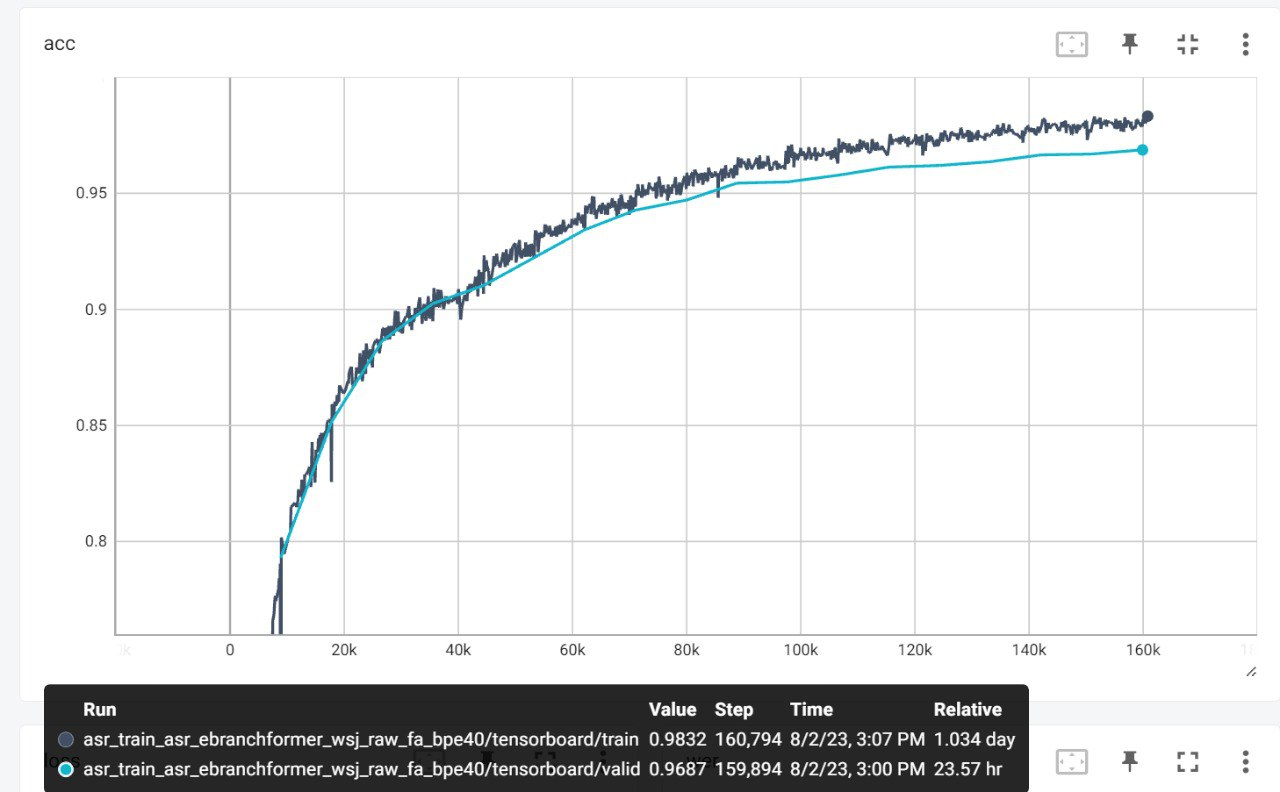
\includegraphics[width=1.1\linewidth, 
                    height=0.25\textheight]
                    {Images/Chapter3/train2.jpg}
			\caption{دقت مدل}
			\label{Acc}
		\end{subfigure}\hfil % <-- added
		\begin{subfigure}{0.5\textwidth}
			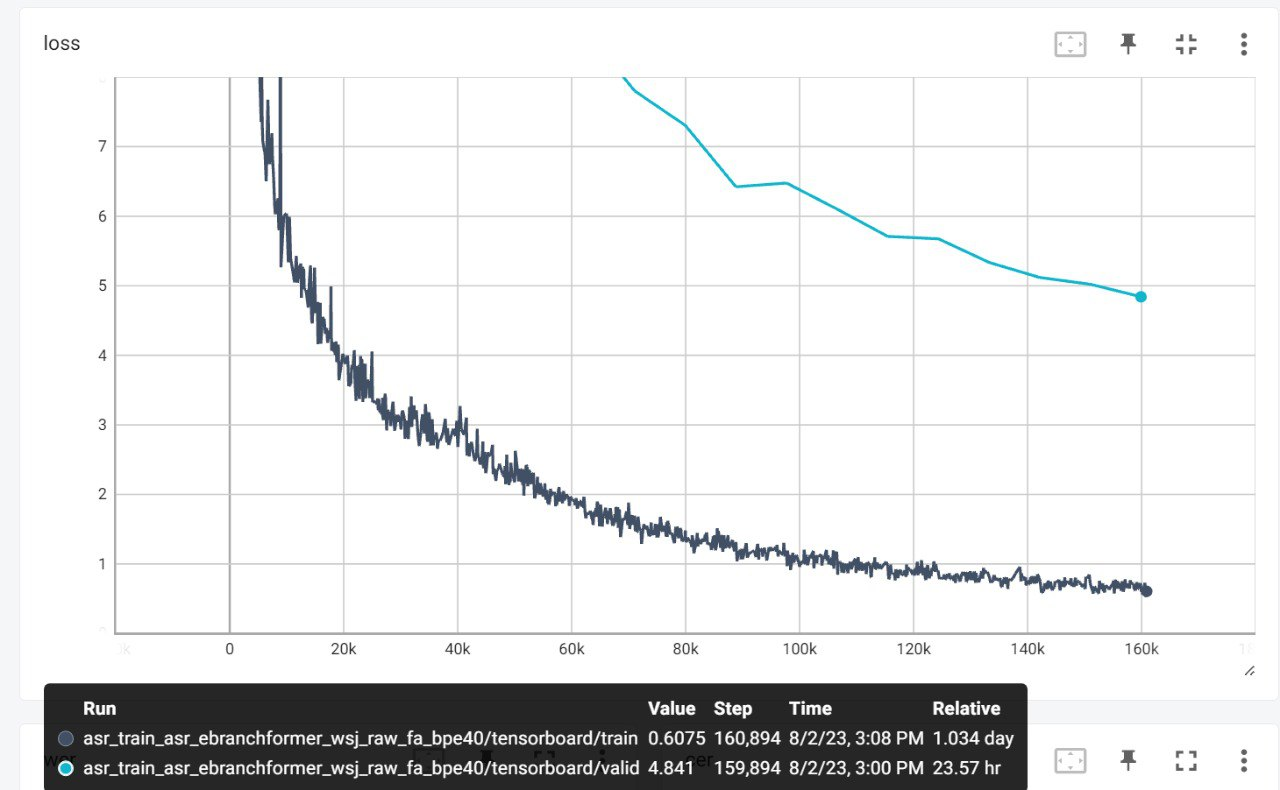
\includegraphics[width=1.1\linewidth, 
                height=0.25\textheight]
                {Images/Chapter3/train3.jpg}
			\caption{مقدار تابع هزینه مدل}
			\label{Cost}
		\end{subfigure}\hfil % <-- added
		\begin{subfigure}{0.5\textwidth}
			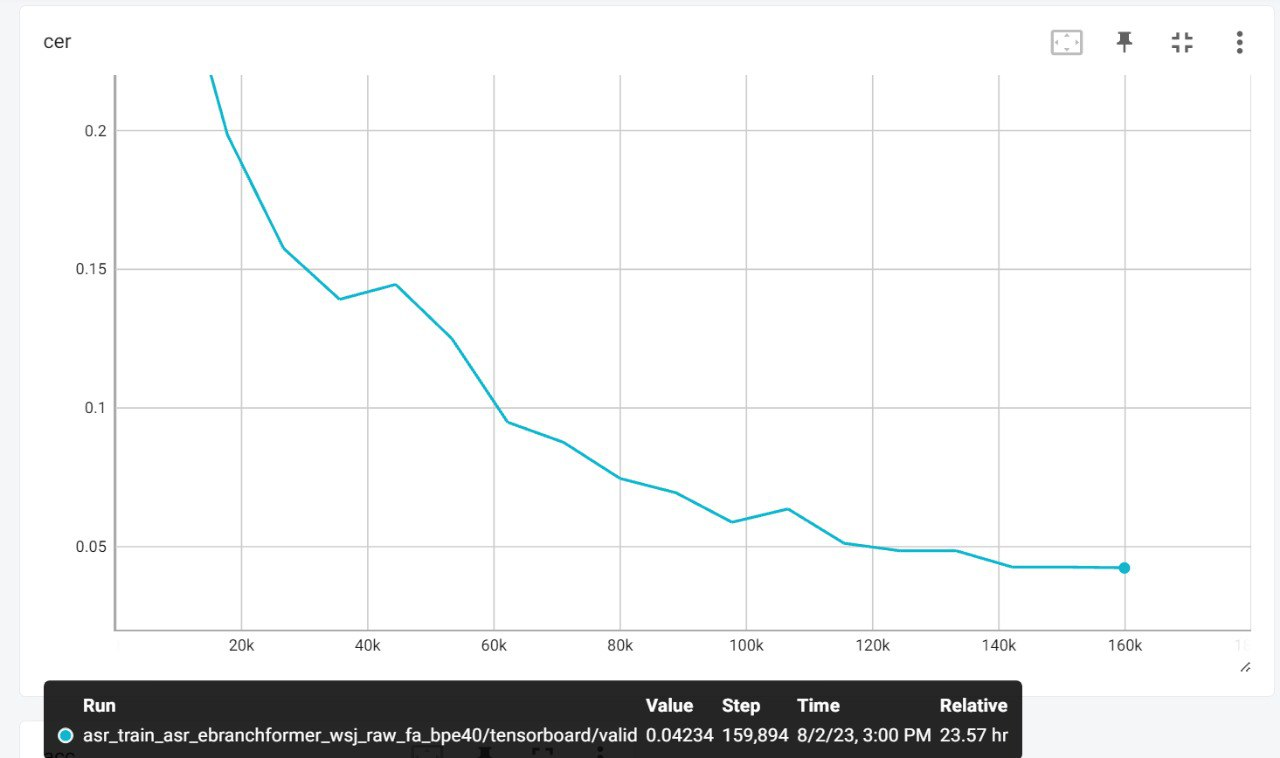
\includegraphics[width=1.1\linewidth, 
                height=0.25\textheight]
                {Images/Chapter3/train4.jpg}
			\caption{مقدار خطای حروف مدل}
			\label{CER}
		\end{subfigure}\hfil % <-- added
		\begin{subfigure}{0.5\textwidth}
			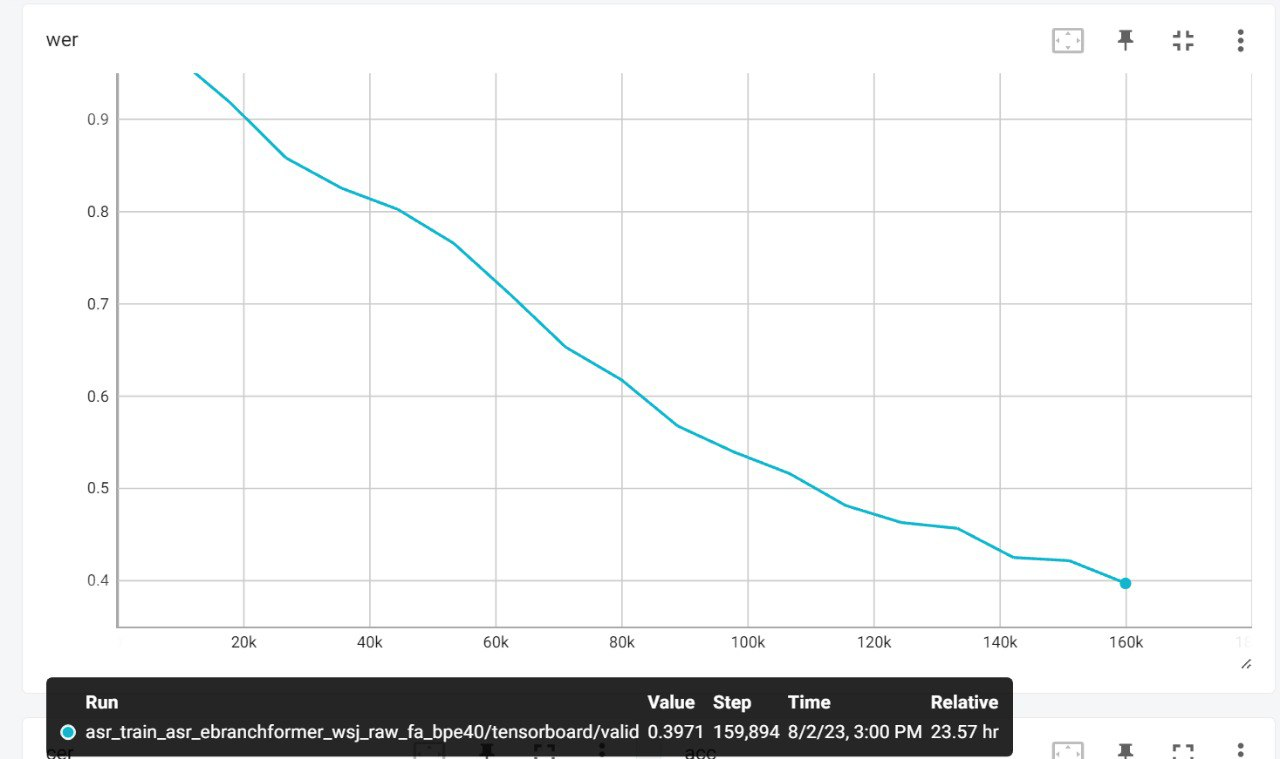
\includegraphics[width=1.1\linewidth, 
                height=0.25\textheight]
                {Images/Chapter3/train5.jpg}
			\caption{مقدار خطای کلمه مدل}
			\label{WER}
		\end{subfigure}
		\caption{تصاویر مربوط به روند آموزش مدل صوت شنانسی بازشناسی گفتار 
  فارسی. این تصاویر خروجی تنسوربرد می‌باشند.}
		\label{fig:train}
\end{figure}

شکل \ref{fig:train} روند آموزش مدل صوت شنانسی را نمایش می‌دهد.
این تصاویر با استفاده تنسوربرد\LTRfootnote{Tensor Board} ایجاد شده اند که درک روند آموزش مدل را با تصاویر و گزارشاتی که ارائه می‌کند بسیار راحت می‌کند.\cite{tensorflow2015-whitepaper}
همین طور که از تصاویر مشخص است مدل روند بسیار پایداری در طول آموزش داشته است و خروجی بسیار رضایت بخش می‌باشد. برای نرخ خطای حروف\LTRfootnote{CER: Character Error Rate}
مقدار $0.04$ بر روی دیتای های ولیدیشن\LTRfootnote{Validation}
بدست آمده است.
و همچنین مقدار $0.397$ درصد برای نرخ خطای کلمه\LTRfootnote{WER: Word Error Rate} بدست آمده است.
نرخ خطا کلمه و حروف
از مهمترین متریک های ارزیابی مدل های بازشناسی گفتار می‌باشند که نتایج حاصله با توجه به حجم دادگان و نوع آنها بسیار رضایت بخش می‌باشد.

برای آموزش این مدل همان طور که مقاله ای-برانچفرمر تاکید کرده است \cite{kim2022ebranchformer}
از دستورعمل های پیش فرض 
یی-اس-پی نت
استفاده شده است اما در مواردی که نیاز به تغییر جزئیات به منظور مناسب سازی برای زبان فارسی بوده است کد ها به صورت دستی تغییر داده شده‌اند. در با توجه به نبود هیچ دوره و آموشی در مورد آموزش دادن مدل زبانی با 
یی-اس-پی نت
وجود نداشت به استفاده از مدل صوت شنانسی اکتفا شده اما در مراحل بعد یک مدل زبانی برای مدل آموزش داده شده است که خروجی آن را بهبود ببخشد.

\section{بررسی خروجی و رفع ایرادات}

همانطور که پیشتر اشاره شد در بازشناسی گفتار یک مدل زبانی به کنار یک مدل صوت شنانسی قرار می‌گیرد که درک گفتار و نوشتار آن به بهترین حالت ممکن صورت بپذیرد با این حال می‌توان از مدل صوت شنانسی به تنهایی برای این منظور استفاده کرد که باعث کاهش دقت زبانی گفتار رونویسی شده می‌شود. با این حال در این مرحله مدل صوت شنانسی را بر روی دادگان تست دیکد کردم تا خروجی تست آن را بررسی کینم.

\begin{figure}[H]
  \centering
  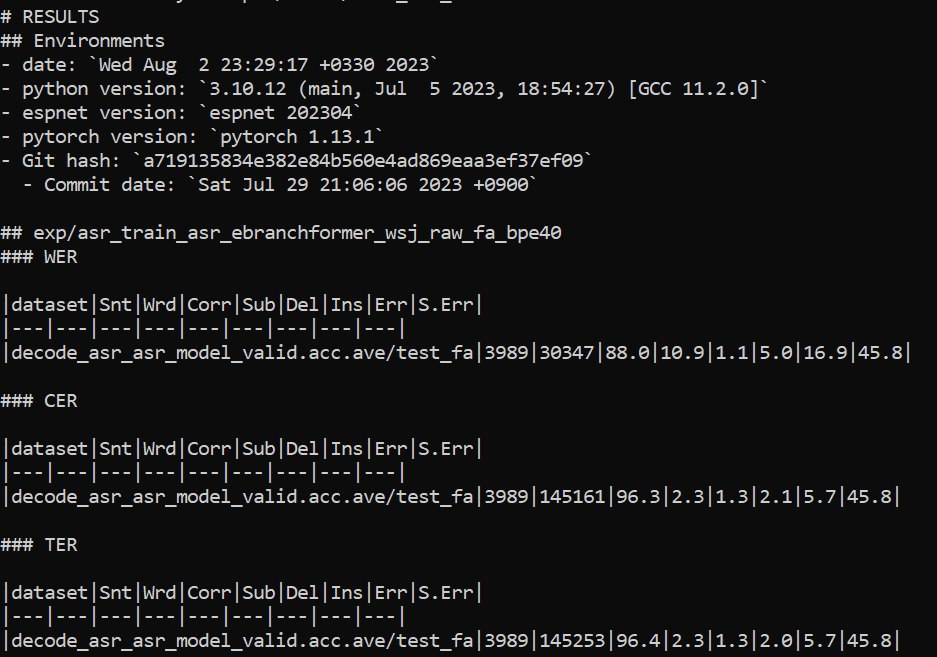
\includegraphics[width=1\textwidth,height=7cm]{Images/Chapter3/decode.jpeg}
  \caption{
  نتایج دیکد مدل صوت شنانسی بدون مدل زبانی بر روی دادگان تست کامن ویس
  }
  \label{fig:decode1}
\end{figure}

شکل \ref{fig:decode1} خروجی مدل را بر روی دادگان تست کامل ویس نشان می‌دهد.
مقدار نرخ خطای کلمه $16.9$ برای کاربرد های امروز نرخ بالایی است اگرچه وجود یک مدل زبانی کنار مدل صوت شنانسی می‌تواند این نرخ خطا را تا نصف کاهش دهد با این حال در کاربرد های امروزی این نرخ بالایی می‌باشد.

در ادامه روند آموزش توسط ارشد پروژه مورد بررسی قرار گرفت و تعدادی از ایرادات که مرتبه اول آموزش مرتکب شدم شناسایی شد و برای اصلاح آنها تلاش شد. در ادامه به تعدادی از مهم ترین این خطاها و راهکار هایی که برای اصلاح آنها انجام دادم اشاره خواهد شد؛ پس از اصلاح این ایرادات مدل دوباره آموزش داده شد و نتایج بسیار ارزشمندی حاصل شد.
\subsection{اشتباه در انتخاب درست تعداد مجموعه توکن ها}
بعد از بررسی هایی که توسط تیم انجام شد یکی از اشتباهات من در طول آموزش انتخاب اشتباه تعداد اعضای مجموعه توکن ها بود.
در ابزار یی-اس-پی نت استیج پنجم آموزش در بازشناسی گفتار باید مجموعه توکن های مشخص شود. زمانی که از مدل های
توجه
استفاده می‌شود باید توکن لیستی از حروف زبان فارسی ایجاد شود که مدل هر آوایی را به یک توکن متناظر\LTRfootnote{Map} کند و رونویسی زبان فارسی را یادبگیرد.
این کار می‌تواند به سه نوع در یی-اس-پی نت انجام شود.

\begin{enumerate}

  \item بر اساس حروف: در این حالت مجموعه توکن ها حروف های زبان فارسی می‌باشد

  \item بر اساس کلمات: در این حالت مجموعه توکن ها بر اساس کلمات زبان فارسی می‌باشد

  \item براساس مدل \texttt{\raggedright bpe}: در حالت ترکیبی از کلمات و حروف ها برای زبان فارسی ایجاد می‌شود.

\end{enumerate}

برای زبان فارسی با توجه به تکراری بودن بعضی از ترکیبات کلمات در اکثر جملات فارسی بهتر است که از 
\verb|bpe|
استفاده شود.
برای استفاده از این نوع ایجاد کننده توکن باید به ابزار یه سری اطلاعات بدهیم. برای مثال باید تعداد اعضای مجموعه توکن ها را با مشخص کردن مقدار متغییر 
\verb|nbpe|
انجام دهیم. برای مثال اگر مقدار این متغییر را 150 بگذاریم خود ابزار ای-ای-پی نت برای ما لیستی از 150 توکن (که تعدادی از آنها حروف و تعدادی دیگر کلمه می‌باشند) ایجاد می‌کند و آن را در یک فایل به نام \verb|tokens.txt|
ذخیره می‌کند. این فایل بعدا توسط مدل برای آموزش استفاده می‌شود.

من در بار اول آموزش اشتباها مقدار
\verb|nbpe|
را 40 گذاشتم ولی در واقع مقدار استاندارد آن 150 می‌باشد و این کار باعث شده بود بعضی از حروف مانند "ژ" در مجموعه توکن های نباشد. این امر باعث کاهش شدید دقت مدل  شده بود و پس از اصلاح آموزش را دوباره آغاز کردم و نتایج جدید بدست آمد.
\begin{figure}[H]
		\centering % <-- added
		\begin{subfigure}{0.5\textwidth}
			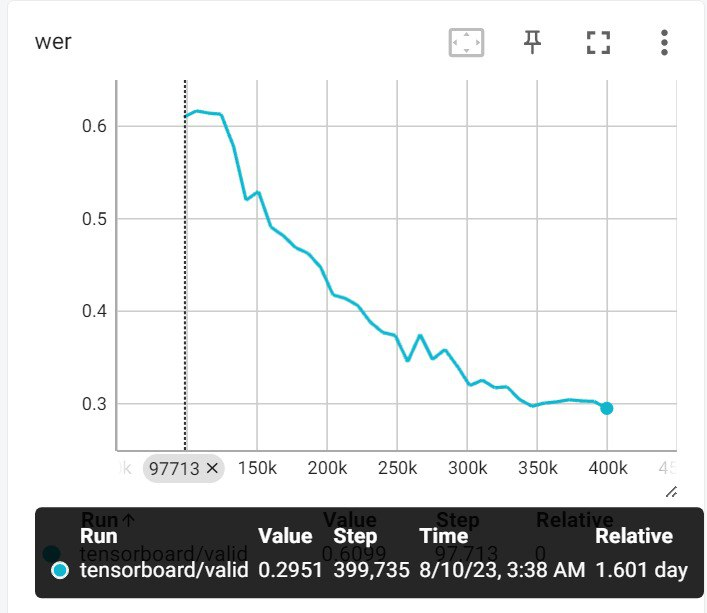
\includegraphics[width=1.1\linewidth, height=0.25\textheight]{Images/Chapter3/train1501.jpg}
			\caption{نرخ خطا  کلمه بر روی ولیدیشن}
			\label{f1}
		\end{subfigure}\hfil % <-- added
		\begin{subfigure}{0.5\textwidth}
			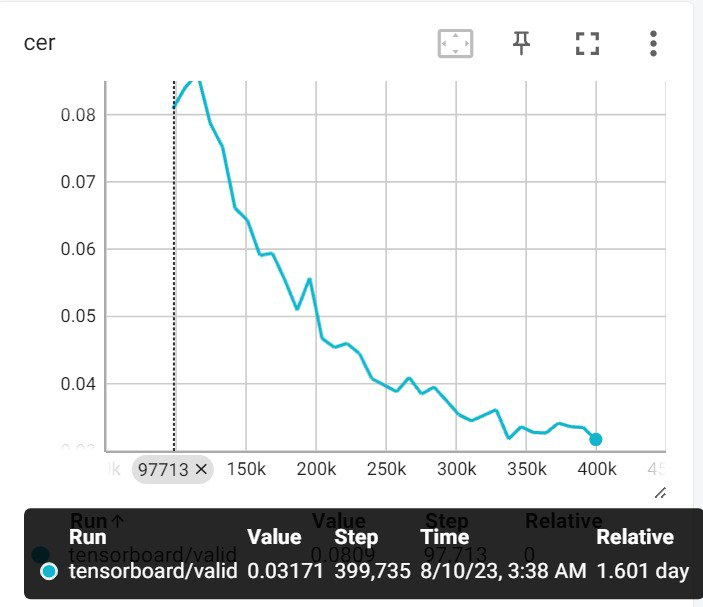
\includegraphics[width=1.1\linewidth, height=0.25\textheight]{Images/Chapter3/train1502.jpg}
			\caption{نرخ خطا حروف بر روی ولیدیشن}
			\label{f2}
		\end{subfigure}\hfil % <-- added
		\label{fig:train150}
            \caption{نمودار های روند آموزش و خروجی آنها بر روی مجموعه ارزیابی با 150 توکن}
\end{figure}
همین طور که در تصویر \ref{f2} و \ref{f1}مشخص است بعد از اعمال تغییرات متریک های مدل بر روی ولیدیشن بهتر شده است. همچنین بر روی تست ست هم خروجی دوبرابر بهتر شده و نرخ خطای کلمات به 8 درصد رسیده است.

\subsection{عدم استفاده از کل داده ها}
با توجه به اینکه روند پیش پردازش داده ها بر روی 
\verb|CPU|
انجام می‌شود و باید تمام فایل های صوتی تغییر فرمت داده شوند من نتوانستم در اولین مرتبه آموزش از کل داده ها استفاده کنم زیرا پیش پردازش کل داده ها روی آن سرور بسیار ارزشمند بود و از بخشی از داده های استفاده کردم. تعداد کم داده ها باعث کاهش دقت مدل شده است و در آموزش جدید از یک سرور با 
\verb|CPU|
قدرتمند تر استفاده شد و خروجی ها بسیار بهبود یافت.

\subsection{عدم استفاده از مدل زبانی}
همانطور که گفته شده برای بهرمندی از بهترین حالت ممکن خروجی باید مدل صوت شنانسی و زبانی کنار هم آموزش داده شوند و استفاده شوند. به همین منظور در این مرحله داده های یک مدل زبانی ترانسفرمری (که در نقش دیکدر در بازشناسی گفتار استفاده می‌شود) بر روی دادگان کامن ویس فارسی آموزش داده شد.آموزش این مدل نصف روز زمان برد. و در نهایت مدل نهای ( که شامل مدل صوت شناسی و زبانی است) بر روی دادگان تست کامن ویس فارسی دیکد شده‌اند و نتایج زیر حاصل شده‌اند.

\begin{figure}[H]
  \centering
  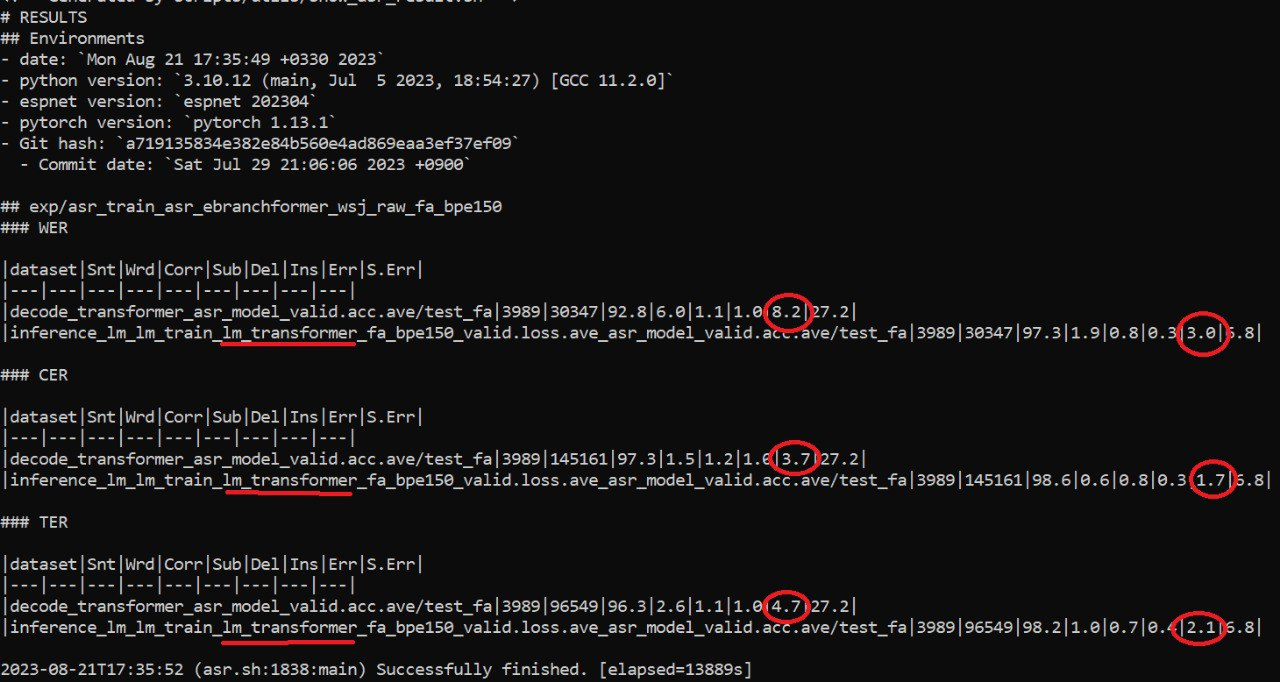
\includegraphics[width=1\textwidth,height=7cm]{Images/Chapter3/decode_best.jpeg}
  \caption{
  نتایج دیکد مدل صوت شنانسی به همراه مدل زبانی بر روی دادگان تست کامن ویس فارسی
  }
  \label{fig:decode_best}
\end{figure}

نتایجی که تصویر \ref{fig:decode_best}
نمایش می‌دهد بسیار عالی و رضایت بخش است. من موفق شدم به نرخ خطای 3 درصد در دادگان تست کامن ویس برسم که این نتیجه در کاربرد فعلی بازشناسی گفتار بسیار عالی می‌باشد. بعد از رسیدن به این نتیاج عالی خروجی مدل در یک جلسه خدمت دکتر صامتی و بقیه اعضای آزمایشگاه نمایش داده شد و مورد قدردانی و تشویق همه اعضا قرار گرفت.

در مرحله بعد کار باید مدل بر روی سرورها پیاده سازی شود که جزئیات مربوط به آن در بخش بعدی بیان خواهد شد.

\section{فراگیری مباحث مورد نیاز برای پیاده سازی بر روی سرور}

در این مرحله کار باید مدل ساخته شده بر روی یک سرور پیاده سازی شود تا بتوان از آن به عنوان یک سرویس جدید برای شرکت استفاده کرد. برای مرحله اول ابتدا باید یک نمونه ساده پیاده سازی شود تا خروجی کار و سرعت عملکرد آن بررسی شود. در ادامه به بررسی چند روش برای پیاده سازی مدل بر روی بک‌اند سرور پرداختم که در نهایت به این نتیجه رسیدم که استفاده از فریم ورک گرادیو\LTRfootnote{Gradio} آسان ترین و سریع ترین راه پیاده سازی مدل های هوش مصنوعی بر روی بک‌اند سرور می‌باشد.\LTRfootnote{ \url{https://github.com/gradio-app/gradio}}


گرادیو
یک کتابخانه پایتون منبع باز است که برای ساخت دموهای یادگیری ماشین و علوم داده و برنامه های کاربردی وب استفاده می شود.
با 
گرادیو
، می توانید به سرعت یک رابط کاربری زیبا در اطراف مدل های یادگیری ماشین یا گردش کار علم داده خود ایجاد کنید و به افراد اجازه دهید با کشیدن و رها کردن در تصاویر خود، چسباندن متن، ضبط صدای خود و تعامل با آن، آن را امتحان کنند.\cite{abid2019gradio}

\section{پیاده سازی بر روی سرور}
در این مرحله از پروژه من اقدام به پیاده سازی مدل بر روی گرادیو کردم. یکی از بزرگترین چالش های این بخش فهمیدن این مسئله بود که چگونه می‌توانیم از مدل آموزش دیده در گرادیو استفاده کنم. با نبود هیچ آموزش و داکیومنتشن در این رابطه من مجبور شدم که دوباره تمام کد های یی-اس-پی نت را بررسی کنم تا در نهایت موفق به پیدا کردن و استفاده از فایل های مربوط به این زمینه در یی-اس-پی نت شدم.
گرادیو را می‌توان به راحتی در هر سروری پیاده سازی کرد ولی برای استفاده عمومی باید سرور قابلیت هاستینگ را داشته باشد. به همین منظور از سرور های هاگینگ فیس\LTRfootnote{Hugging Face} برای پیاده سازی مدل  استفاده شده است.\LTRfootnote{\url{https://github.com/huggingface} , \url{https://huggingface.co/}}

هاگینگ فیس یک شرکت فرانسوی-آمریکایی است که ابزارهایی را برای ساخت برنامه های کاربردی با استفاده از یادگیری ماشین، مستقر در شهر نیویورک توسعه می دهد. این به خاطر کتابخانه ترانسفورماتورهای خود که برای برنامه های کاربردی پردازش زبان طبیعی ساخته شده است و پلتفرم آن که به کاربران اجازه می دهد مدل ها و مجموعه داده های یادگیری ماشین را به اشتراک بگذارند و کار خود را در یک فضا به نمایش بگذارند قابل توجه است.\cite{wolf2020huggingfaces}

بعد از یادگیری کار با هاگینگ فیس و گرادیو موفق شدم نسخه اولیه نرم سرویسی باز شناسی گفتار فارسی را پیاده سازی کنیم. برای دسترسی به این نرم افزار بررسی آن کافی است بر روی این \href{https://huggingface.co/spaces/parsa-mhmdi/persian-asr}{لینک} کلیک کنید.
ر این نرم افزار امکان ضبط فایل صدا و همچینین ارسال فایل صوتی وجود دارد و پس از چند ثانیه پردازش نرم افزار متن گفته شده در فایل صوتی را بازنویسی می‌کند.\LTRfootnote{ \url{https://huggingface.co/spaces/parsa-mhmdi/persian-asr}}
با تمام تلاش های صورت گرفته این نرم افزار همچنان در مرحله توسعه می‌باشد و هنوز آماده کار های تجاری نشده است برای کار های حرفه ای همچنان به کار های بیشتر نیاز دارد. با توجه به اینکه سرور های رایگان هاگینگ فیس فقط اجازه استفاده از
\verb|CPU|
می‌دهد ممکن زمان پردازش مقداری طولانی تر از \verb|GPU|
باشد.

\begin{figure}[H]
  \centering
  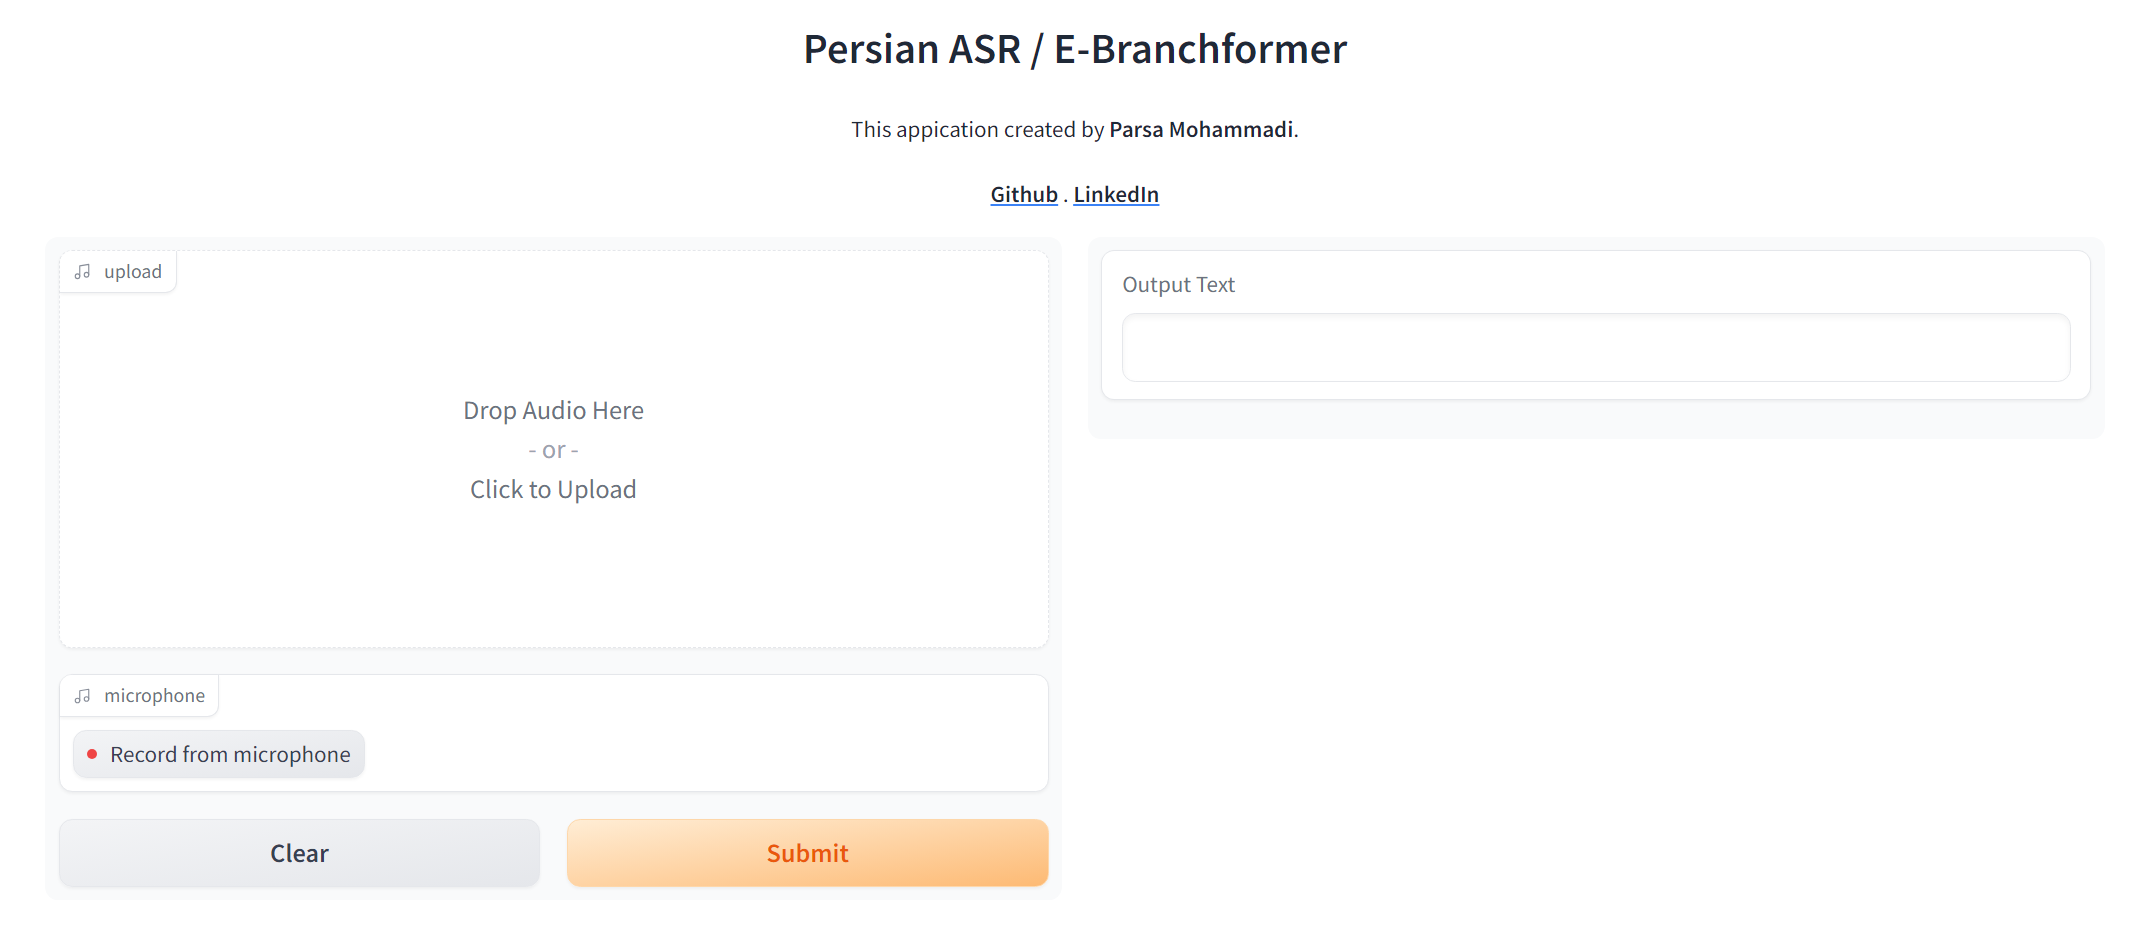
\includegraphics[width=1\textwidth,height=7cm]{Images/Chapter3/UI.png}
  \caption{
  تصویر رابط کاربری نرم افزار بازشناسی گفتار فارسی 
  }
  \label{fig:UI}
\end{figure}

\section{مستندسازی و ارائه خروجی}
در نهایت کار خلاصه از تمام انجام شده و نتایج حاصل شده مستند سازی شده و در جلسه آزماشیگاه ارئه شد. دکتر صامتی ضمن قدردانی پیشنهاد پیاده سازی این مدل بازشناسی گفتار برای زبان عربی را دادند که در صورت ادامه همکاری با شرکت این پروژه برای کارفرمای مربوطه انجام شود. در ادامه تمام کد ها گزاش ها و مدل های آموزش داده شده خدمت شرکت تسلیم شد و بر روی ریپازیتوری کارآموزش قرار گرفت.

بعد از اتمام این تجربه دلنشین و بسیار آموزنده کارآموزی نامه های مربوط به گذراندن 240 ساعت کارآموزی با امضای مدیرعامل شرکت دریافت شد و یک لوح تقدیر به من داده شد. تمام این مدارک در انتهای این گزارش کارآموزی پیوست شده است.











\chapter{جمع‌بندي و نتيجه‌گيري و پیشنهادات}
%%%%%%%%%%%%%%%%%%%%%%%%%%%%%%%%%%%%%%%%%%%
در این فصل با توجه مباحثی که در فصل های قبل بیان شد و تجارب ارزشمندی که کسب شد به نتیجه‌گیری و پیشنهادات این پروژه کارآموزی اشاره خواهد شد.

\section{نتیجه‌گیر و جمع‌بندی}

همانطور که در فصل های گذشته بیان شد مدل های بازشناسی گفتار امروز کاربرد های زیادی دارند اما با اینکه چندین سرویس بازشناسی گفتار فارسی موجود است امّا هیچ کدام از آنها از مدل های جدید خودنگرش\LTRfootnote{Self-attention} استفاده نمی‌کنند؛ این امر باعث شده است در بعضی موارد ضعیف عمل کنند. من در دوره با راهنمایی ارشد پروژه و کمک های استاد راهنمای کارآموزی دکتر سیدین سرپرست کارآموزی دکتر بیراوند موفق و شدم یک مدل بازشناسی گفتار فارسی با دقت بسیار بالا درست کنم.

در نهایت این سرویس بازشناسی گفتار فارسی بر روی سرور های شرکت و سرور های هاگینگ فیس پیاده سازی شد و در حال حاظر نسخه اولیه آن در دسترس عموم می‌باشد. این مدل جدید توانایی درک کلمات جدید و پیچیده را دارد و می‌تواند به درستی رو نویسی کند امکانی که در مدل های قبلی فراهم نبود.

با این حال برای رسیدن به نسخه نهایی و استفاده در صنعت نیازمند استفاده  دیتاست های بزرگتر و با دامنه گفتار گسترده تر می‌باشد. همچنین استفاده از مدل زبانی بزرگ هم میتواند در بهبود عملکرد این مدل نقش به سزایی ایفا کند.


\section{پیشنهادات}
همان طور پیشتر گفته شد تعداد بیشتر دادگان می‌تواند باعث افزایش هرچه بیشتر دقت سرویس شود. به این منظور استفاده از داده های گفتاری که شامل لهجه های مختلف، صدا های پس زمینه مختلف و گوینده هایی با بازه سنی بیشتر است می‌تواند دقت سرویس بازشناسی گفتار فارسی را بسیار افزایش دهد.

پیشنهاد دیگری که می‌توان برای این پروژه ارائه کرد استفاده مدل هایی با معماری بزرگتر و پارامتر های بیشتر می‌باشد. برای این پروژه بخاطر محدودیت در امکانات محسباتی من مجبور شدم که از معماری متوسط ای-برانچفرمر متوسط استفاده کنم که بتوان با وجود حافظه کم واحد پردازش گرافیکی مدل را آموزش دهم. اما اگر سخت افزار های قوی تر با توان محاسباتی و حافظه بیشتر موجود باشد می‌توان مدل ای-برانچفرمر بزرگ را آموزش داد و دقت خروجی را بالا برد.

به عنوان آخرین پیشنهاد می‌توان استفاده مدل های زبانی بزرگ\LTRfootnote{Large Language Model} را مطرح کرد.
تحقیقات جدید نشان می‌دهند که می‌توان یک مدل زبانی بزرگ را بر روی حجم زیادی از دادگان آموزش داد و از آن برای تمام کار های پردازش گفتار و متن استفاده کرد و نتایج خوبی دریافت کرد.\cite{huang2023language} باتوجه به اینکه در بازشناسی گفتار از مدل زبانی و مدل صوت شناسی کنار هم استفاده می‌شود بنظر می‌آید که مدل زبانی قوی می‌تواند ضعف مدل صوت شناسی را جبران کند و خروجی هایی با دقت بالا تولید کند.


%--------------------------------------------------------------------------appendix( مراجع و پیوست ها)
\renewcommand{\bibname}{منابع و مراجع}
\chapterfont{\vspace*{-2em}\centering\LARGE}%

\appendix
\bibliographystyle{unsrt-fa}
\bibliography{references}
\chapter*{‌پیوست}
\markboth{پیوست}{}
\addcontentsline{toc}{chapter}{پیوست}
در این بخش نامه های مربوط کارآموزی پیوست شده است.

\begin{figure}[H]
  \centering
  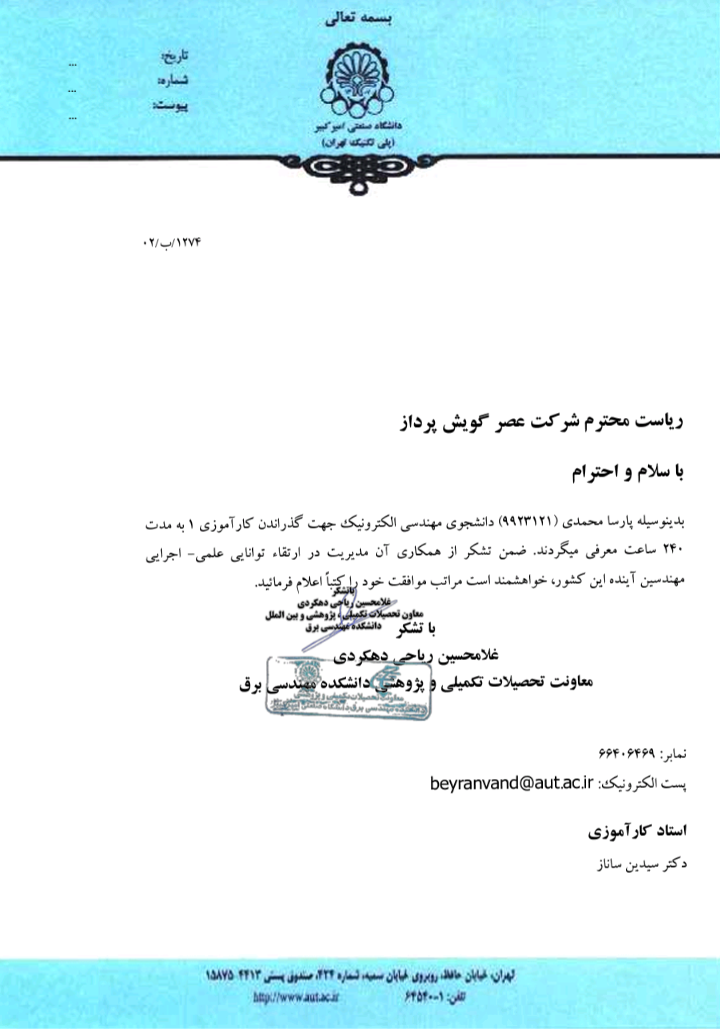
\includegraphics[width=1\textwidth,height=15cm]{letters/riahi_letter.png}
  \caption{
   نامه ارسال شده توسط دکتر ریاحی به صنعت جهت معرفی کارآموز به شرکت
  }
  \label{img:riahi_letter}
\end{figure}

\begin{figure}[H]
  \centering
  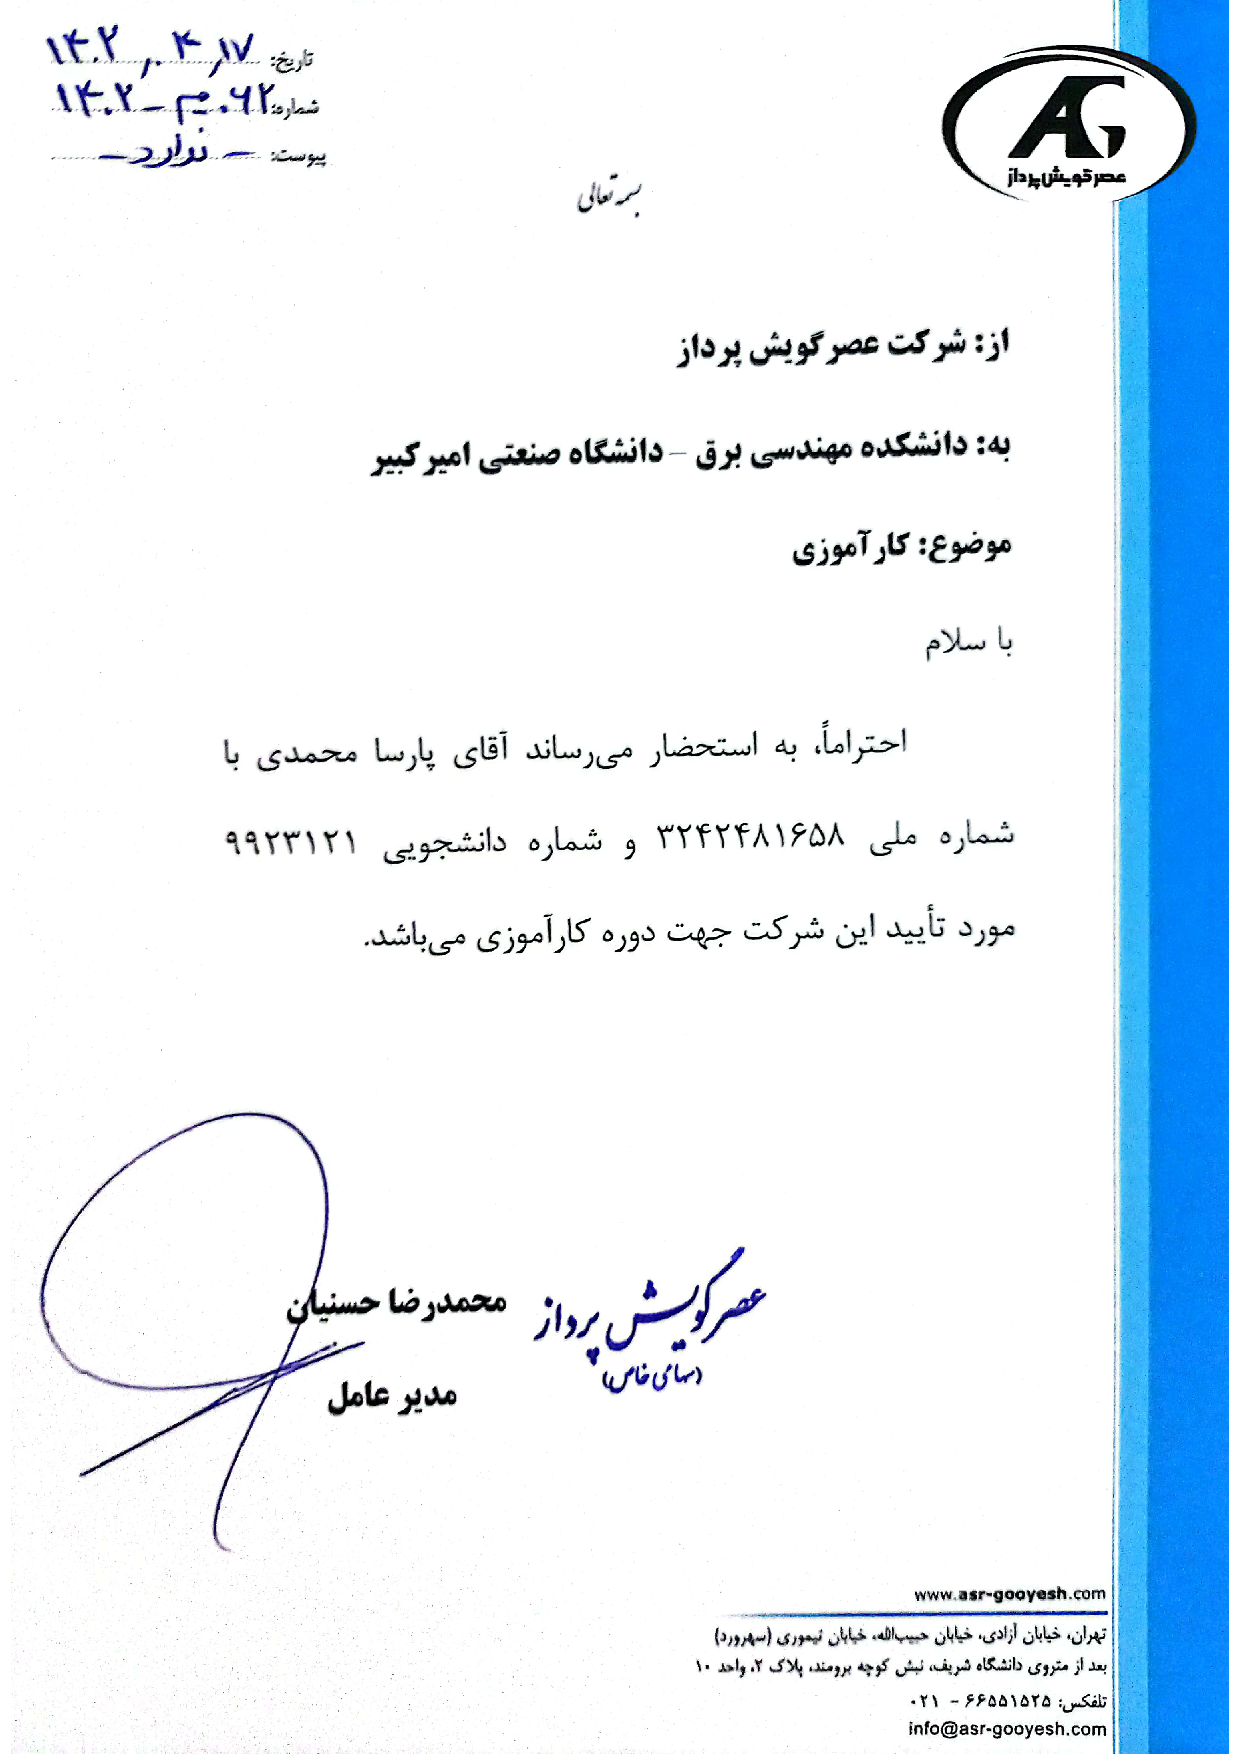
\includegraphics[width=1\textwidth]{letters/riahi_anwser.pdf}
  \caption{
  پاسخ شرکت به نامه دکتر ریاحی و علام موافقت شرکت
  }
  \label{img:riahi_anwser}
\end{figure}

\begin{figure}[H]
  \centering
  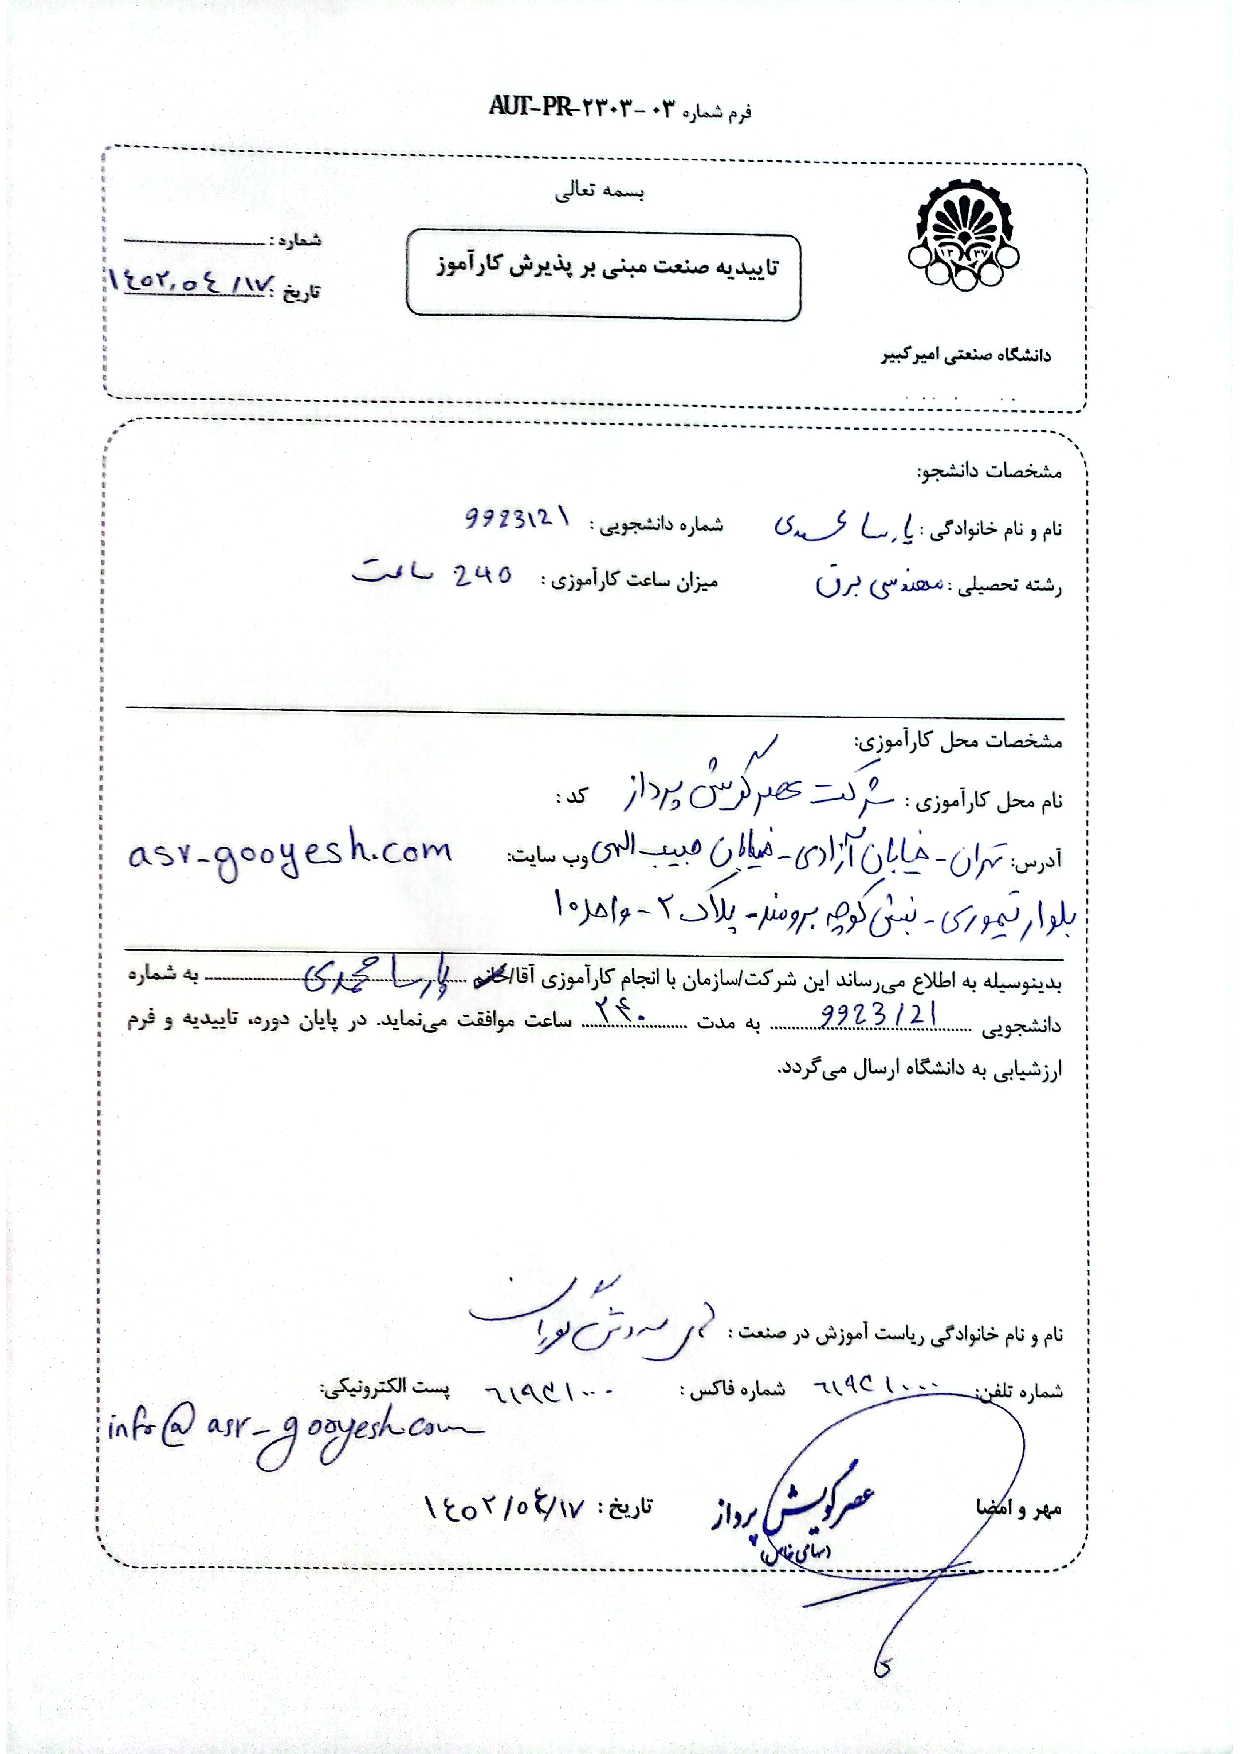
\includegraphics[width=1\textwidth]{letters/taeed_sanaat.pdf}
  \caption{
    فرم تایید صنعت مبنی بر پذیرش کارآموز
  }
  \label{img:taeed_sanaat}
\end{figure}

\begin{figure}[H]
  \centering
  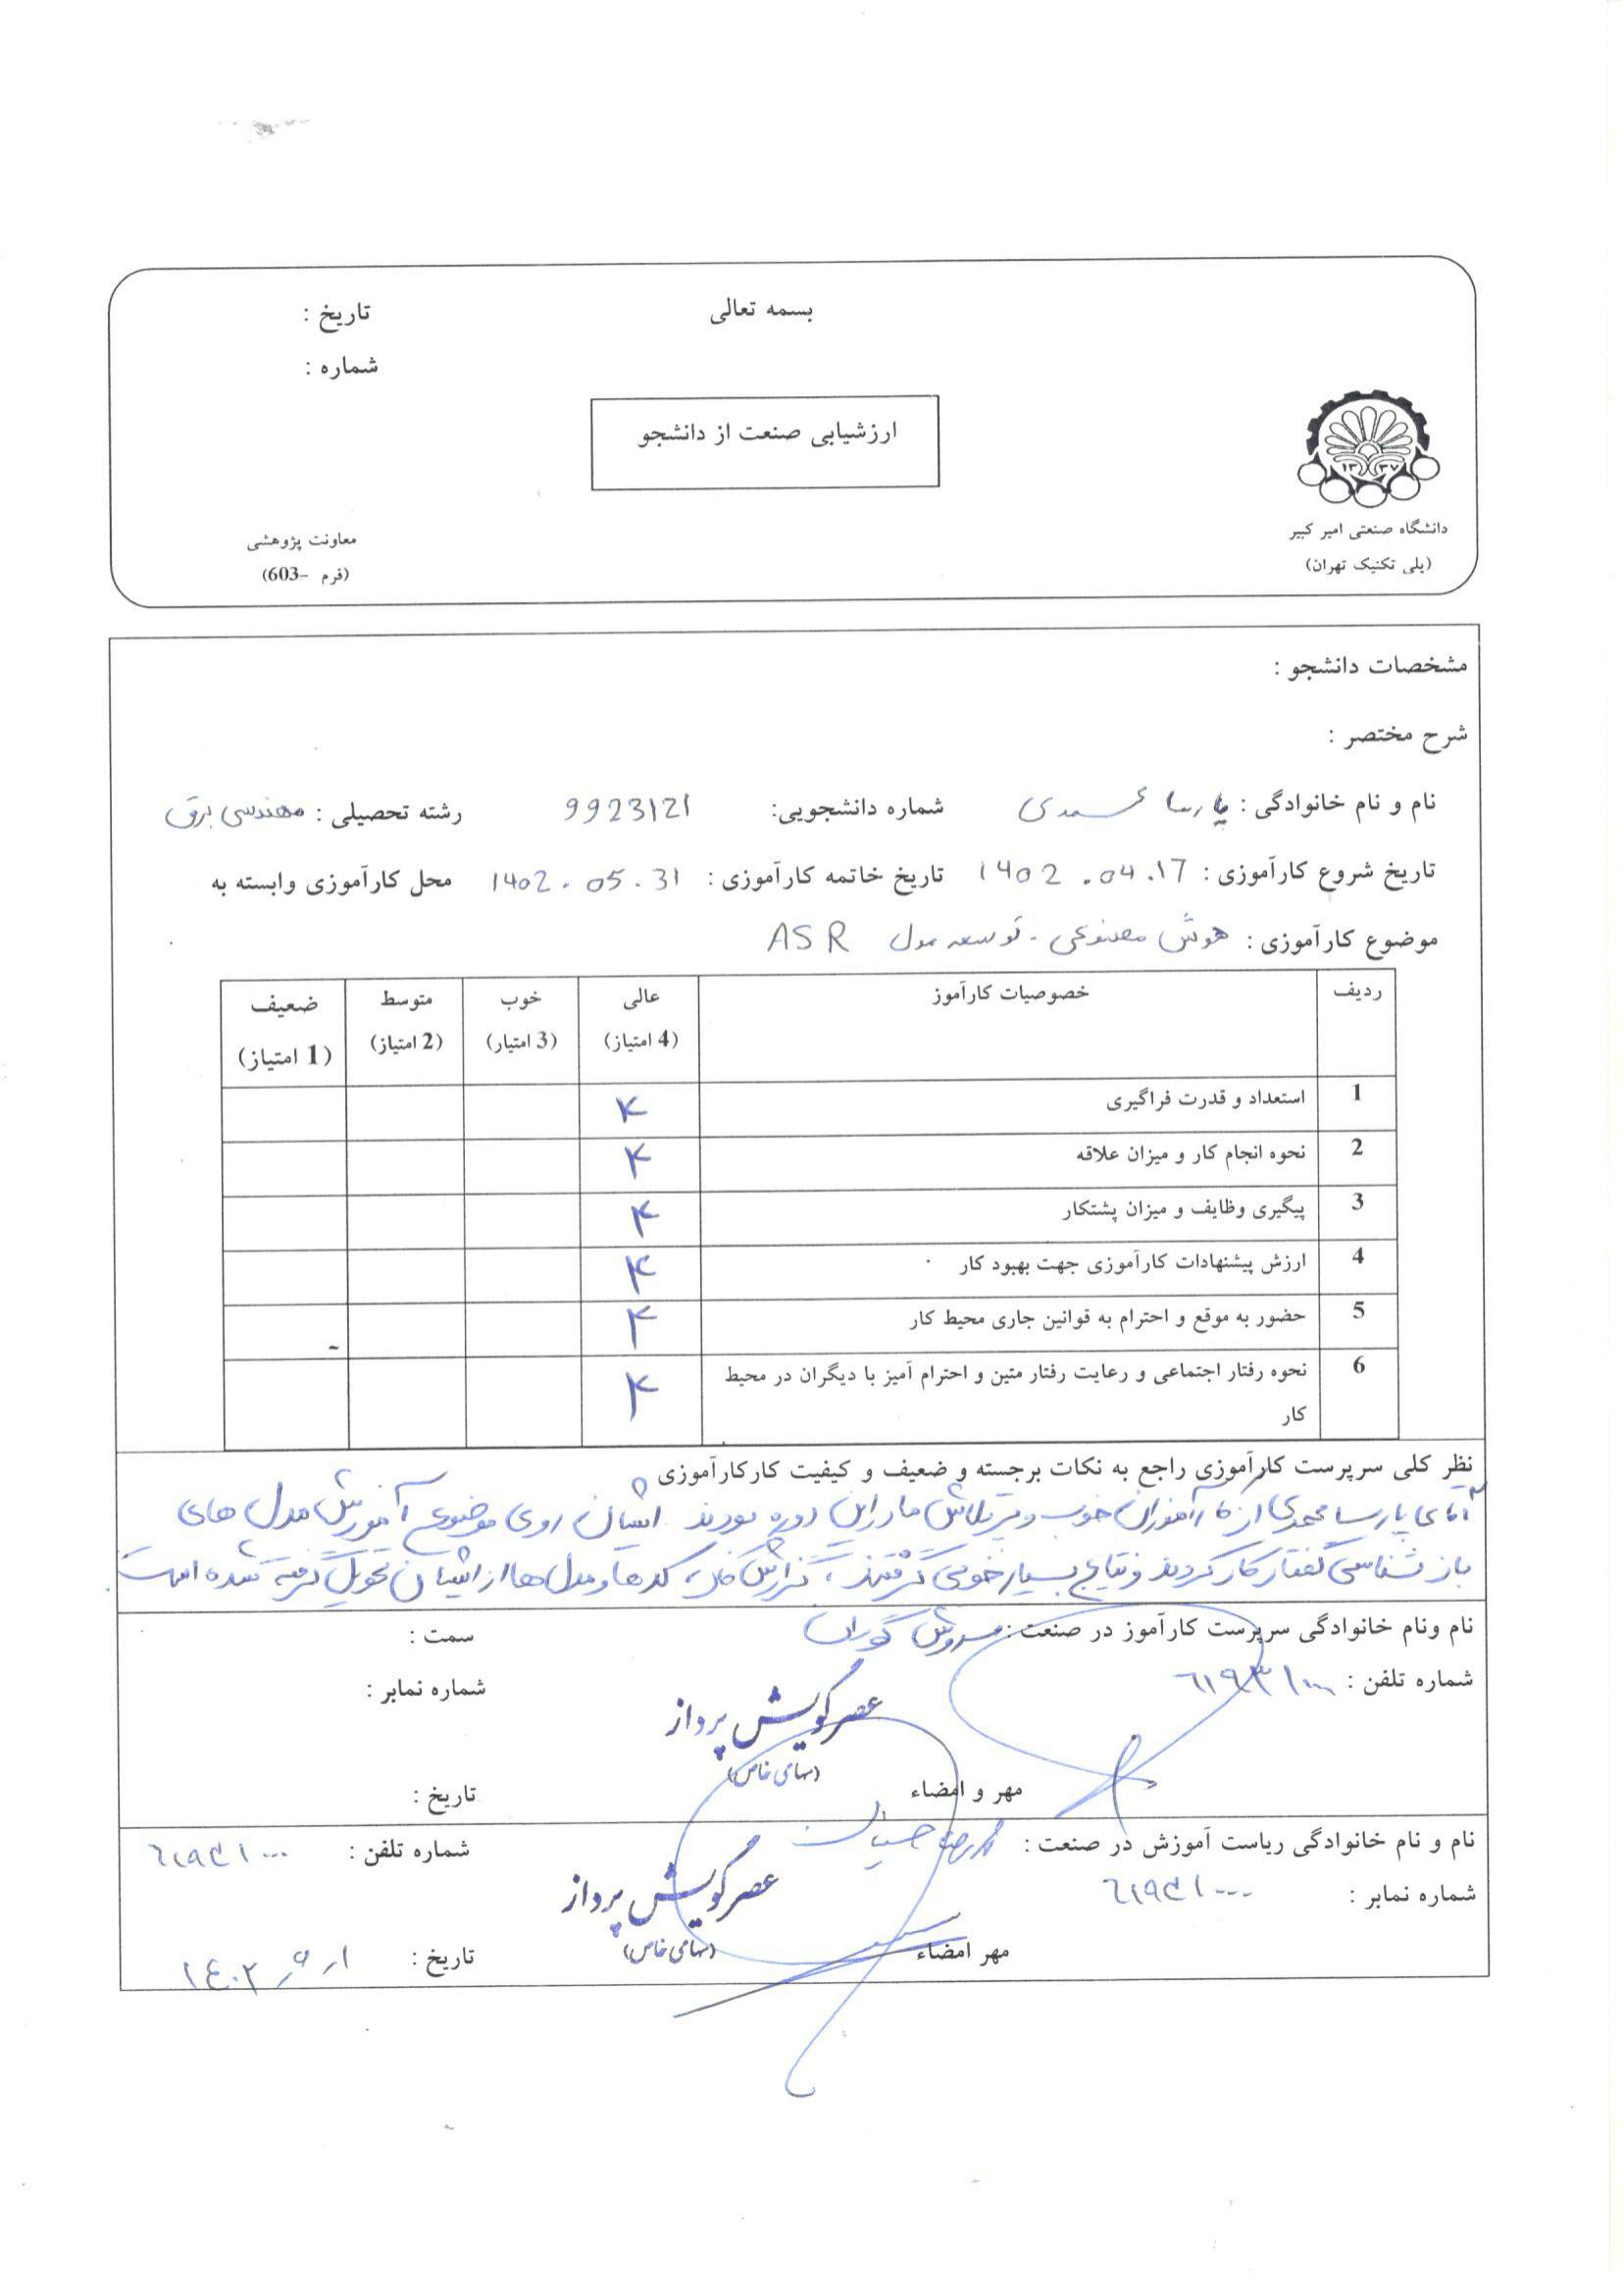
\includegraphics[width=1\textwidth]{letters/arzyabi.jpg}
  \caption{
    فرم ارزیابی صنعت از دانشجو
  }
  \label{img:arzyabi}
\end{figure}

\begin{figure}[H]
  \centering
  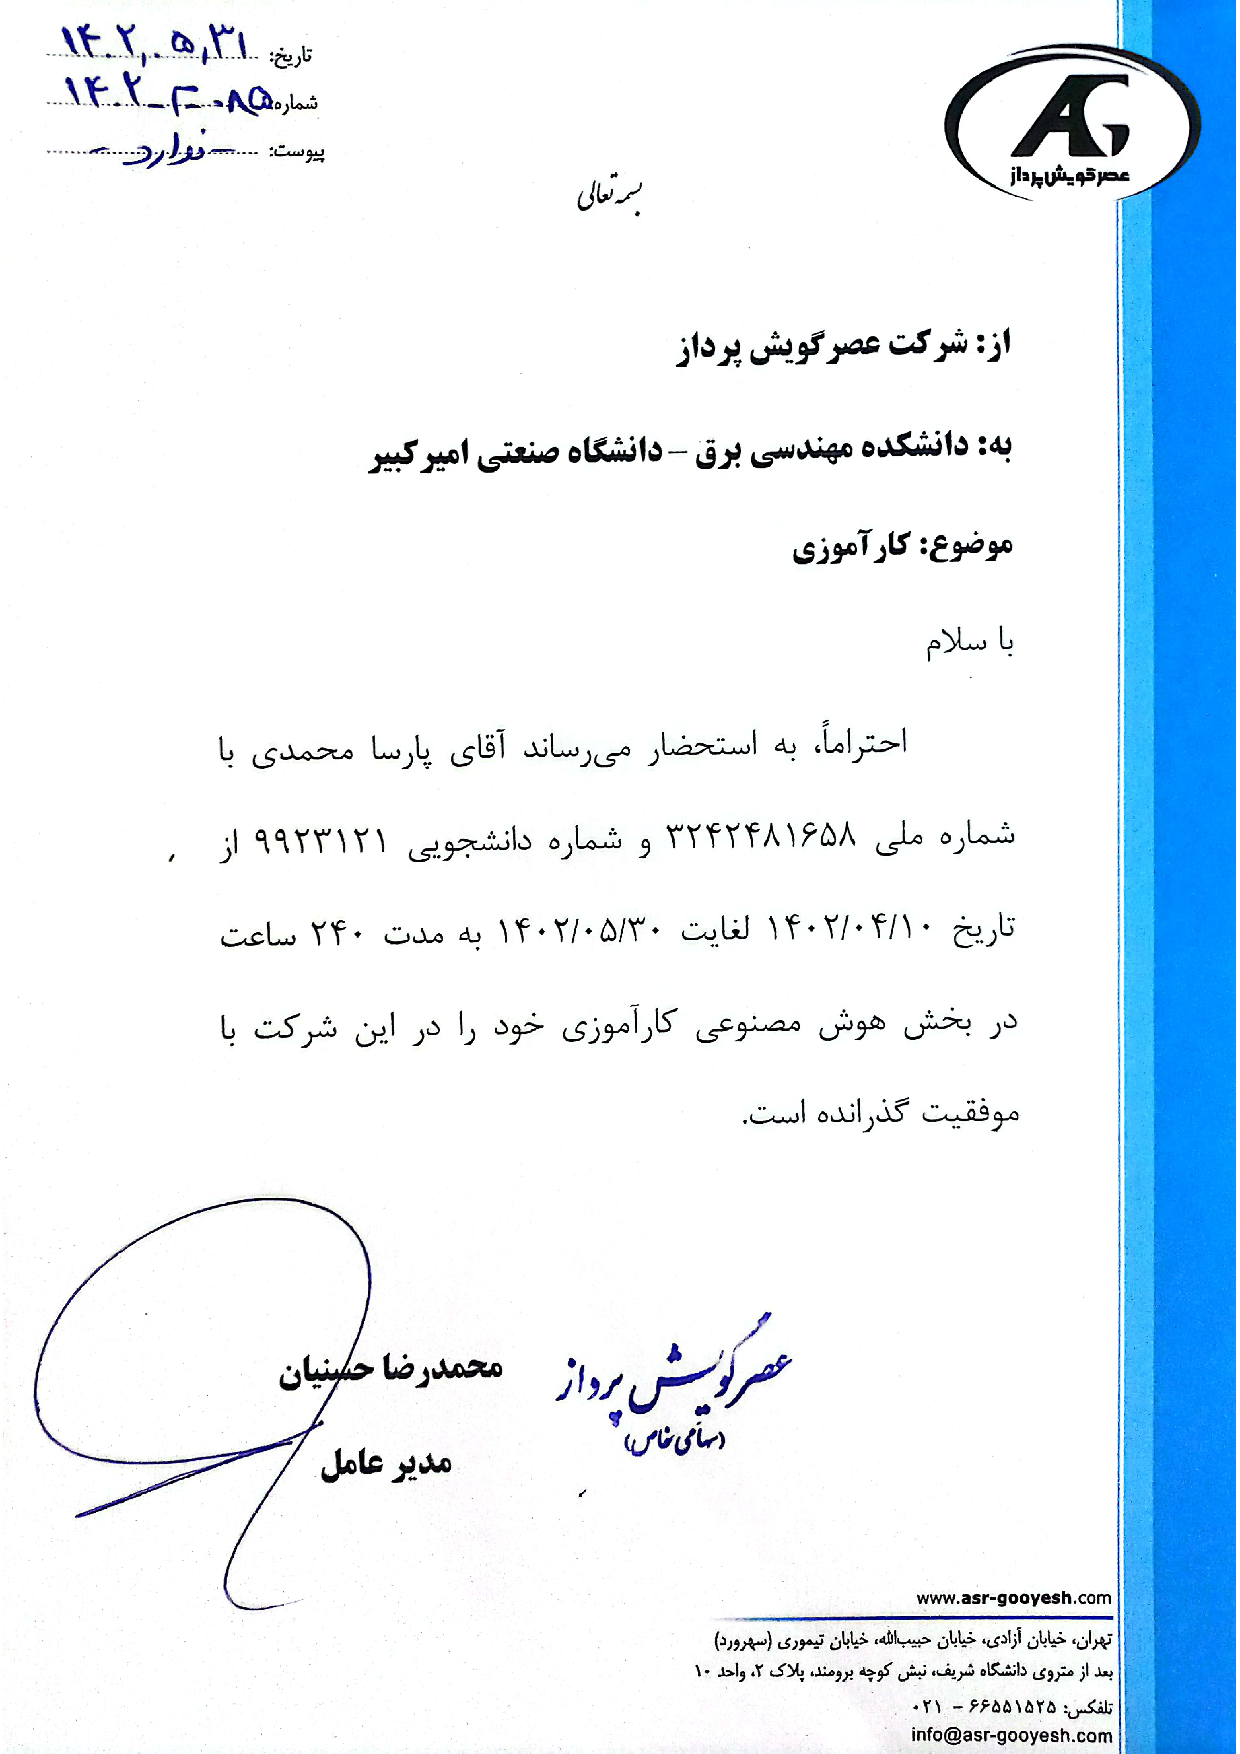
\includegraphics[width=1\textwidth]{letters/240.pdf}
  \caption{
    نامه پایان 240 ساعت کارآموزی در شرکت عصر گویش پرداز
  }
  \label{img:240}
\end{figure}

\begin{figure}[H]
  \centering
  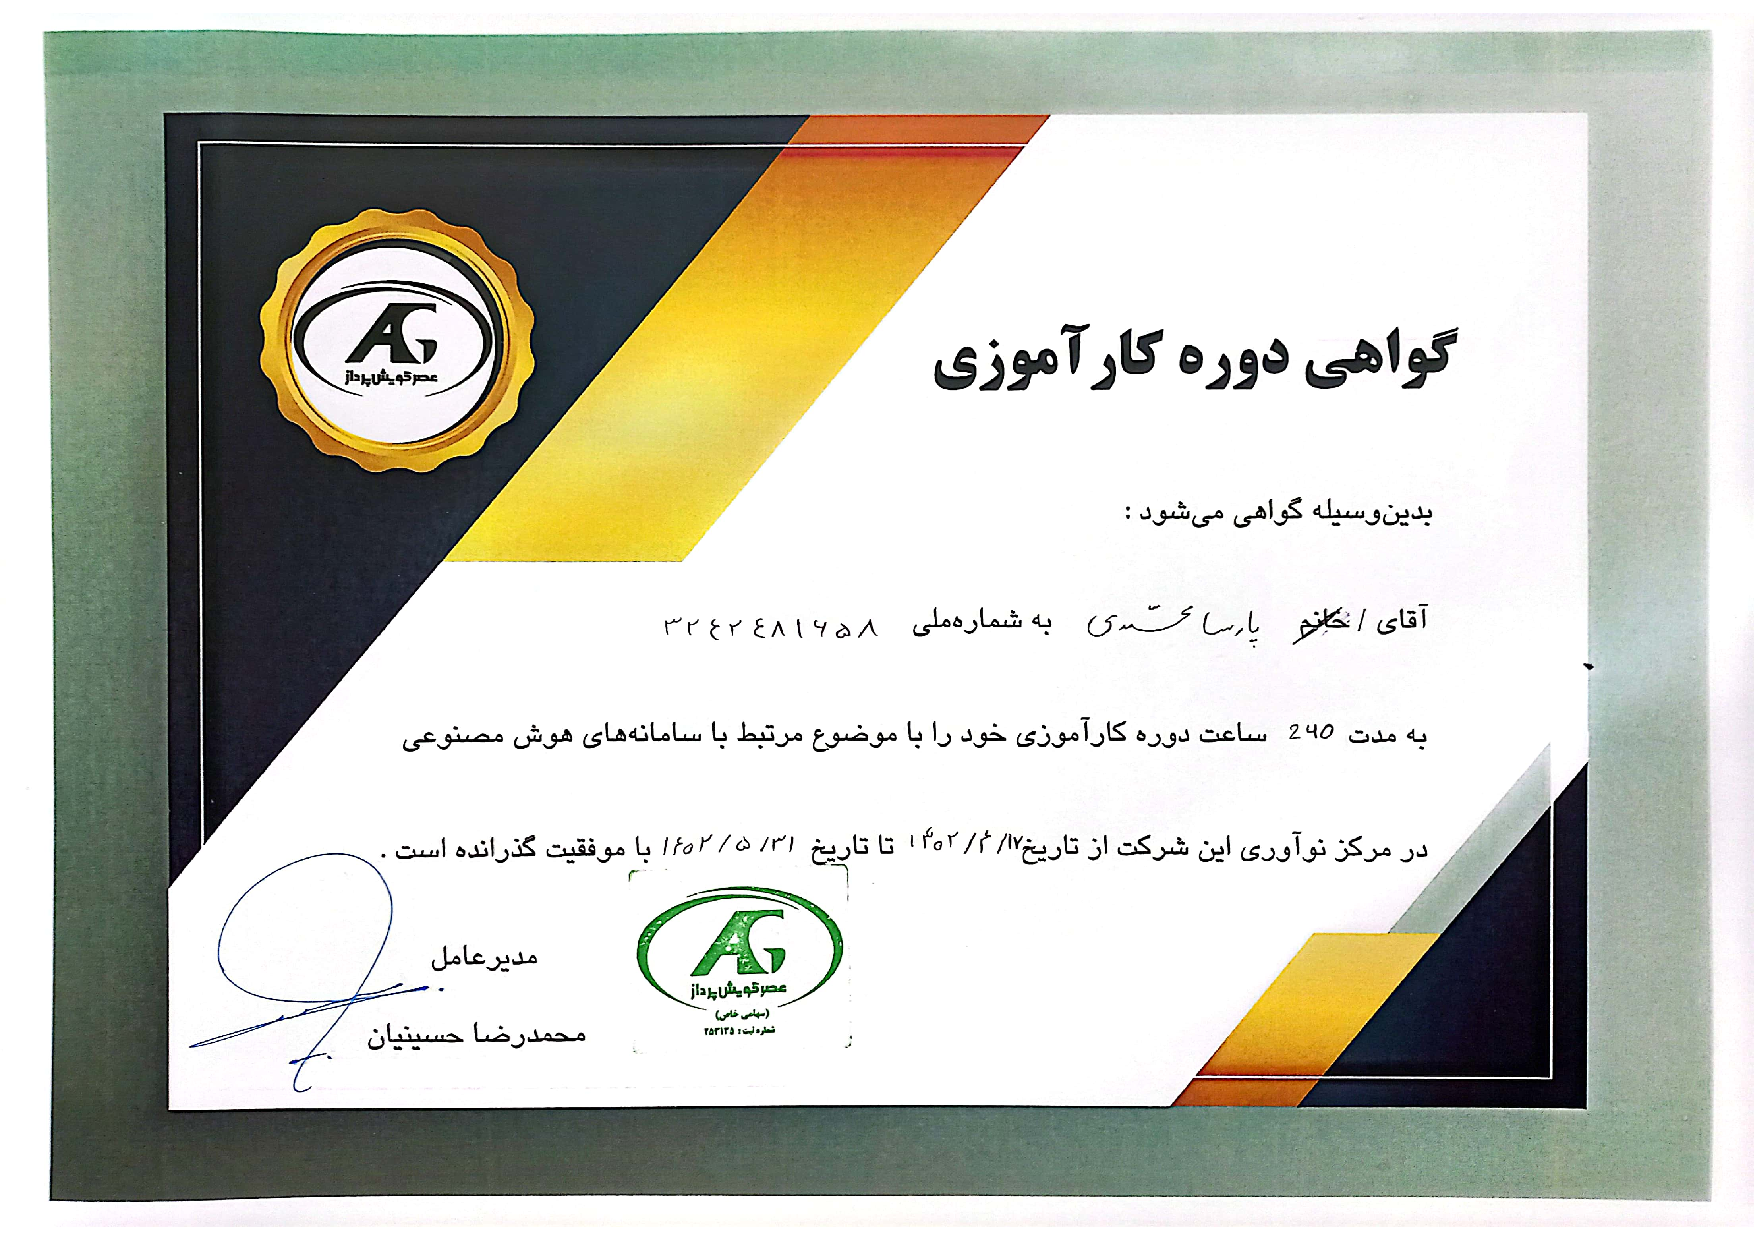
\includegraphics[width=1\textwidth,scale=4]{letters/certificate.pdf}
  \caption{
    گواهی شرکت در دوره کارآموزی شرکت عصر گویش پرداز
  }
  \label{img:certificate}
\end{figure}
%--------------------------------------------------------------------------dictionary(واژه نامه ها)
%اگر مایل به داشتن صفحه واژه‌نامه نیستید، خط زیر را غیر فعال کنید.
\parindent=0pt
% %
\chapter*{واژه‌نامه‌ی فارسی به انگلیسی}
\pagestyle{style9}

\addcontentsline{toc}{chapter}{واژه‌نامه‌ی فارسی به انگلیسی}
%%%%%%
\begin{multicols*}{2}

% {\bf آ}
% \vspace*{3mm}


% \farsiTOenglish{اسکالر}{Scalar}


\vspace*{3mm}
{\bf ب}
\vspace*{3mm}

\farsiTOenglish{بازشناسی خودکار گفتار}{Automatic Speech Recognition}
\farsiTOenglish{برخط}{Online}


% \vspace*{3mm}
% {\bf پ}
% %%\vspace*{3mm}

% \farsiTOenglish{پایا}{Invariant}



\vspace*{3mm}
{\bf ت}
%%\vspace*{3mm}

\farsiTOenglish{ ترانسفورمر }{Transformer}


% \vspace*{3mm}
% {\bf ث}
% %%\vspace*{3mm}

% \farsiTOenglish{ثابت‌ساز}{Stabilizer}

% \vspace*{3mm}
% {\bf ج}
% %%\vspace*{3mm}

% \farsiTOenglish{جایگشت}{Permutation}



% \vspace*{3mm}
% {\bf چ}
% %%\vspace*{3mm}


% \farsiTOenglish{چند جمله‌ای }{Polynomial}

% \vspace*{3mm}
% {\bf ح}
% %%\vspace*{3mm}

% \farsiTOenglish{حاصل‌ضرب دکارتی}{Cartesian product}


% \vspace*{3mm}
% {\bf خ}
% %%\vspace*{3mm}

% \farsiTOenglish{خودریختی}{Automorphism}

% \vspace*{3mm}
% {\bf د}
% %%\vspace*{3mm}

% \farsiTOenglish{درجه}{Degree}


% \vspace*{3mm}
% {\bf ر}
% %%\vspace*{3mm}


% \farsiTOenglish{ریزپردازنده}{microprocessor}


% \vspace*{3mm}
% {\bf ز}
% %%\vspace*{3mm}


% \farsiTOenglish{زیرمدول}{Submodule}


% \vspace*{3mm}
% {\bf س}
% %%\vspace*{3mm}

% \farsiTOenglish{سرشت}{Character}


% \vspace*{3mm}
% {\bf ص}
% %%\vspace*{3mm}

% \farsiTOenglish{صادقانه}{Faithful}

% \vspace*{3mm}
% {\bf ض}
% %%\vspace*{3mm}

% \farsiTOenglish{ضرب داخلی}{Inner product}

% \vspace*{3mm}
% {\bf ط}
% %%\vspace*{3mm}


% \farsiTOenglish{طوقه}{Loop}


% \vspace*{3mm}
% {\bf ظ}
% %%\vspace*{3mm}


% \farsiTOenglish{ظرفیت}{Valency}
 
% \vspace*{3mm}
% {\bf ع}
% %%\vspace*{3mm}


% \farsiTOenglish{عدم مجاورت}{Nonadjacency}



% \vspace*{3mm}
% {\bf ف}
% %%\vspace*{3mm}

% \farsiTOenglish{فضای برداری}{Vector space}



% \vspace*{3mm}
% {\bf ک}
% %%\vspace*{3mm}

% \farsiTOenglish{کاملاً تحویل‌پذیر}{Complete reducibility}


% \vspace*{3mm}
% {\bf گ}
% %%\vspace*{3mm}


% \farsiTOenglish{گراف}{Graph}



% \vspace*{3mm}
% {\bf م}
% %%\vspace*{3mm}

% \farsiTOenglish{ماتریس جایگشتی}{Permutation matrix }


% \vspace*{3mm}
% {\bf ن}
% %%\vspace*{3mm}

% \farsiTOenglish{ناهمبند}{Disconnected}


% \vspace*{3mm}
% {\bf و}
% %%\vspace*{3mm}

% \farsiTOenglish{وارون‌پذیر}{Invertible}


% \vspace*{3mm}
% {\bf ه}
% %%\vspace*{3mm}

% \farsiTOenglish{همبند}{Connected}



% \vspace*{3mm}
% {\bf ی}
% %%\vspace*{3mm}

% \farsiTOenglish{یال}{Edge}




\end{multicols*}%
%%%%%%
\chapter*{ واژه‌نامه‌ی انگلیسی به فارسی}
\pagestyle{style9}
\lhead{\thepage}\rhead{واژه‌نامه‌ی انگلیسی به فارسی}
\addcontentsline{toc}{chapter}{واژه‌نامه‌ی انگلیسی به فارسی}

\LTRmulticolcolumns
\begin{multicols}{2}
{\hfill\bf  \lr{A}}
\vspace*{1.5mm}

\englishTOfarsi{Automatic Speech Recognition}{بازشناسی خودکار گفتار}
\englishTOfarsi{Acoustics}{صوت شناسی}

\vspace*{3mm}
{\hfill\bf   \lr{B}}
%%\vspace*{1.5mm}

\englishTOfarsi{Batch}{دسته}

\vspace*{3mm}
{\hfill\bf   \lr{C}}
%%\vspace*{1.5mm}

\englishTOfarsi{Convolutional Neural Network}{شبکه‌های عصبی پیچشی}
\englishTOfarsi{Connectionist Temporal Classification}{طبقه بندی زمانی ارتباط گرایانه}
\englishTOfarsi{Character Error Rate}{نرخ خطای حرف}


\vspace*{3mm}
{\hfill\bf   \lr{D}}
%%\vspace*{1.5mm}

\englishTOfarsi{Decoder}{رمز گشا}

\vspace*{3mm}
{\hfill\bf   \lr{E}}
%%\vspace*{1.5mm}

\englishTOfarsi{End to End}{سر‌ به سر، سرهم پیوسته}
\englishTOfarsi{Encoder}{رمز گذار}
\englishTOfarsi{Enhanced}{تقویت شده}


% \vspace*{3mm}
% {\hfill\bf   \lr{F}}
% %%\vspace*{1.5mm}

% \englishTOfarsi{Function}{تابع}

\vspace*{3mm}
{\hfill\bf   \lr{G}}
%%\vspace*{1.5mm}

\englishTOfarsi{Global Optima}{نتقطه بهینه سراسری}
\englishTOfarsi{Global}{جهانی، سراسر}


% \vspace*{3mm}
% {\hfill\bf   \lr{H}}
% %%\vspace*{1.5mm}

% \englishTOfarsi{Homomorphism}{همریختی}

% \vspace*{3mm}
% {\hfill\bf   \lr{I}}
% %%\vspace*{1.5mm}

% \englishTOfarsi{Invariant}{پایا}

\vspace*{3mm}
{\hfill\bf   \lr{L}}
%%\vspace*{1.5mm}

\englishTOfarsi{Local}{محلی}
\englishTOfarsi{Large Language Model}{مدل زبانی بزرگ}

\vspace*{3mm}
{\hfill\bf   \lr{M}}
%%\vspace*{1.5mm}

\englishTOfarsi{Mini-Batch}{کوچک دسته}
\englishTOfarsi{Map}{نگاشت}

\vspace*{3mm}
{\hfill\bf   \lr{N}}
%%\vspace*{1.5mm}

\englishTOfarsi{Natural Language Processing}{پردازش زبان طبیعی}

\vspace*{3mm}
{\hfill\bf   \lr{O}}
%%\vspace*{1.5mm}

\englishTOfarsi{Online}{بر خط}

\vspace*{3mm}
{\hfill\bf   \lr{P}}
%%\vspace*{1.5mm}

\englishTOfarsi{Pipeline}{خط لوله}

% \vspace*{3mm}
% {\hfill\bf   \lr{Q}}
% %%\vspace*{1.5mm}

% \englishTOfarsi{Quotient graph}{گراف خارج‌قسمتی}

 \vspace*{3mm}
{\hfill\bf   \lr{R}}
%%\vspace*{1.5mm}

\englishTOfarsi{Recurrent Neural Network}{شبکه عصبی مکرر}
\englishTOfarsi{Research and Development}{تحقیق و توسعه}
\englishTOfarsi{Recipe}{دستور عمل}

\vspace*{3mm}
{\hfill\bf   \lr{S}}
%%\vspace*{1.5mm}

\englishTOfarsi{Speech Recognition}{بازشناسی گفتار}
\englishTOfarsi{Self Attention}{خود نگرش}
\englishTOfarsi{Semi-Supervised}{نیمه نظارتی}
\englishTOfarsi{Sequence}{دنباله}


 \vspace*{3mm}
{\hfill\bf   \lr{T}}
%%\vspace*{1.5mm}

\englishTOfarsi{Toolkit}{جعبه ابزار}
\englishTOfarsi{Token List}{مجموعه نماد ها، نشان ها}

% \vspace*{3mm}
% {\hfill\bf   \lr{U}}
% %%\vspace*{1.5mm}

% \englishTOfarsi{Unique}{منحصربفرد}

\vspace*{3mm}
{\hfill\bf   \lr{V}}
%%\vspace*{1.5mm}

\englishTOfarsi{Validation}{ارزیابی}

\vspace*{3mm}
{\hfill\bf   \lr{W}}
%%\vspace*{1.5mm}
\englishTOfarsi{Word Error Rate}{نرخ خطای کلمه}
\englishTOfarsi{Word Embedding}{تعبیه کلمات}

\end{multicols}
%--------------------------------------------------------------------------index(نمایه)
%اگر مایل به داشتن صفحه نمایه نیستید، خط زیر را غیر فعال کنید.
% \pagestyle{style7}
% \printindex
% \pagestyle{style7}
% %کلمات کلیدی انگلیسی
\latinkeywords{Write a 3 to 5 KeyWords is essential. Example: AUT, M.Sc., Ph. D,..}
%چکیده انگلیسی

\en-abstract{
This page is accurate translation from Persian abstract into English.
}
%%%%%%%%%%%%%%%%%%%%% کدهای زیر را تغییر ندهید.

\newpage
\thispagestyle{empty}
\begin{latin}
\section*{\LARGE\centering Abstract}

\een-abstract

\vspace*{.5cm}
{\large\textbf{Key Words:}}\par
\vspace*{.5cm}
\elatinkeywords
\end{latin}
% % در این فایل، عنوان پایان‌نامه، مشخصات خود و چکیده پایان‌نامه را به انگلیسی، وارد کنید.
%%%%%%%%%%%%%%%%%%%%%%%%%%%%%%%%%%%%
\baselineskip=.6cm
\begin{latin}

\latinfaculty{Department of ...}


\latintitle{Title of Thesis}


\firstlatinsupervisor{Dr. }

%\secondlatinsupervisor{Second Supervisor}

\firstlatinadvisor{Dr. }

%\secondlatinadvisor{Second Advisor}

\latinname{Name}

\latinsurname{Surname}

\latinthesisdate{Month \& Year}

\latinvtitle
\end{latin}

\end{document}